\documentclass[twoside]{book}

% Packages required by doxygen
\usepackage{fixltx2e}
\usepackage{calc}
\usepackage{doxygen}
\usepackage[export]{adjustbox} % also loads graphicx
\usepackage{graphicx}
\usepackage[utf8]{inputenc}
\usepackage{makeidx}
\usepackage{multicol}
\usepackage{multirow}
\PassOptionsToPackage{warn}{textcomp}
\usepackage{textcomp}
\usepackage[nointegrals]{wasysym}
\usepackage[table]{xcolor}

% Font selection
\usepackage[T1]{fontenc}
\usepackage[scaled=.90]{helvet}
\usepackage{courier}
\usepackage{amssymb}
\usepackage{sectsty}
\renewcommand{\familydefault}{\sfdefault}
\allsectionsfont{%
  \fontseries{bc}\selectfont%
  \color{darkgray}%
}
\renewcommand{\DoxyLabelFont}{%
  \fontseries{bc}\selectfont%
  \color{darkgray}%
}
\newcommand{\+}{\discretionary{\mbox{\scriptsize$\hookleftarrow$}}{}{}}

% Page & text layout
\usepackage{geometry}
\geometry{%
  a4paper,%
  top=2.5cm,%
  bottom=2.5cm,%
  left=2.5cm,%
  right=2.5cm%
}
\tolerance=750
\hfuzz=15pt
\hbadness=750
\setlength{\emergencystretch}{15pt}
\setlength{\parindent}{0cm}
\setlength{\parskip}{3ex plus 2ex minus 2ex}
\makeatletter
\renewcommand{\paragraph}{%
  \@startsection{paragraph}{4}{0ex}{-1.0ex}{1.0ex}{%
    \normalfont\normalsize\bfseries\SS@parafont%
  }%
}
\renewcommand{\subparagraph}{%
  \@startsection{subparagraph}{5}{0ex}{-1.0ex}{1.0ex}{%
    \normalfont\normalsize\bfseries\SS@subparafont%
  }%
}
\makeatother

% Headers & footers
\usepackage{fancyhdr}
\pagestyle{fancyplain}
\fancyhead[LE]{\fancyplain{}{\bfseries\thepage}}
\fancyhead[CE]{\fancyplain{}{}}
\fancyhead[RE]{\fancyplain{}{\bfseries\leftmark}}
\fancyhead[LO]{\fancyplain{}{\bfseries\rightmark}}
\fancyhead[CO]{\fancyplain{}{}}
\fancyhead[RO]{\fancyplain{}{\bfseries\thepage}}
\fancyfoot[LE]{\fancyplain{}{}}
\fancyfoot[CE]{\fancyplain{}{}}
\fancyfoot[RE]{\fancyplain{}{\bfseries\scriptsize Generated by Doxygen }}
\fancyfoot[LO]{\fancyplain{}{\bfseries\scriptsize Generated by Doxygen }}
\fancyfoot[CO]{\fancyplain{}{}}
\fancyfoot[RO]{\fancyplain{}{}}
\renewcommand{\footrulewidth}{0.4pt}
\renewcommand{\chaptermark}[1]{%
  \markboth{#1}{}%
}
\renewcommand{\sectionmark}[1]{%
  \markright{\thesection\ #1}%
}

% Indices & bibliography
\usepackage{natbib}
\usepackage[titles]{tocloft}
\setcounter{tocdepth}{3}
\setcounter{secnumdepth}{5}
\makeindex

% Hyperlinks (required, but should be loaded last)
\usepackage{ifpdf}
\ifpdf
  \usepackage[pdftex,pagebackref=true]{hyperref}
\else
  \usepackage[ps2pdf,pagebackref=true]{hyperref}
\fi
\hypersetup{%
  colorlinks=true,%
  linkcolor=blue,%
  citecolor=blue,%
  unicode%
}

% Custom commands
\newcommand{\clearemptydoublepage}{%
  \newpage{\pagestyle{empty}\cleardoublepage}%
}

\usepackage{caption}
\captionsetup{labelsep=space,justification=centering,font={bf},singlelinecheck=off,skip=4pt,position=top}

%===== C O N T E N T S =====

\begin{document}

% Titlepage & ToC
\hypersetup{pageanchor=false,
             bookmarksnumbered=true,
             pdfencoding=unicode
            }
\pagenumbering{alph}
\begin{titlepage}
\vspace*{7cm}
\begin{center}%
{\Large Lab 9\+: Binary Trees \\[1ex]\large 1 }\\
\vspace*{1cm}
{\large Generated by Doxygen 1.8.12}\\
\end{center}
\end{titlepage}
\clearemptydoublepage
\pagenumbering{roman}
\tableofcontents
\clearemptydoublepage
\pagenumbering{arabic}
\hypersetup{pageanchor=true}

%--- Begin generated contents ---
\chapter{Outputs \& Lab Sheets}
\label{index}\hypertarget{index}{}
\begin{DoxyImageNoCaption}
  \mbox{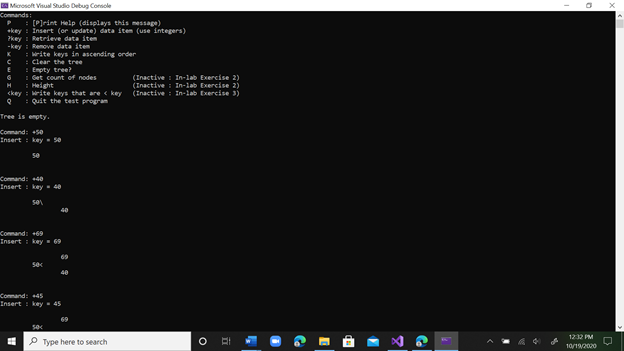
\includegraphics[width=17cm]{Lab9Test1.1.png}}
\end{DoxyImageNoCaption}



\begin{DoxyImageNoCaption}
  \mbox{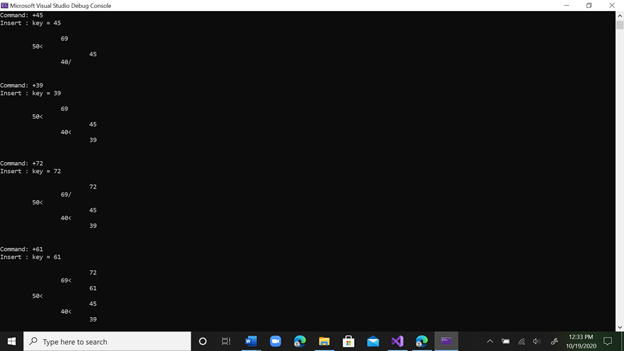
\includegraphics[width=17cm]{Lab9Test1.2.png}}
\end{DoxyImageNoCaption}



\begin{DoxyImageNoCaption}
  \mbox{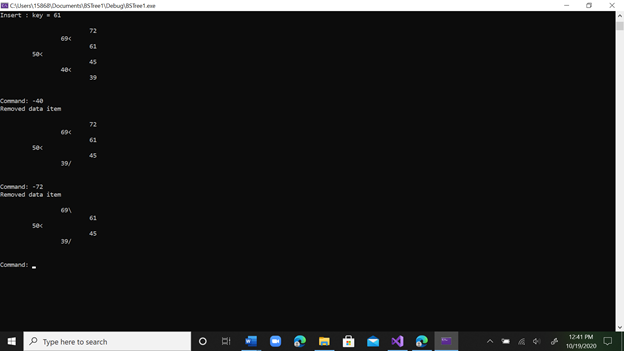
\includegraphics[width=17cm]{Lab9Test1.3.png}}
\end{DoxyImageNoCaption}



\begin{DoxyImageNoCaption}
  \mbox{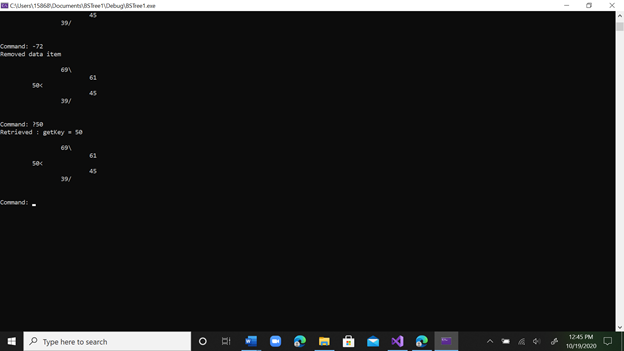
\includegraphics[width=17cm]{Lab9Test1.4.png}}
\end{DoxyImageNoCaption}



\begin{DoxyImageNoCaption}
  \mbox{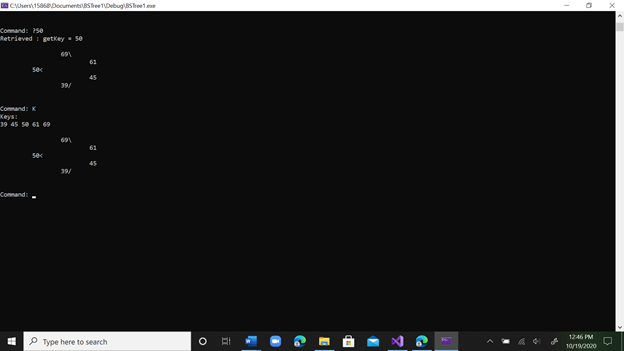
\includegraphics[width=17cm]{Lab9Test1.5.png}}
\end{DoxyImageNoCaption}



\begin{DoxyImageNoCaption}
  \mbox{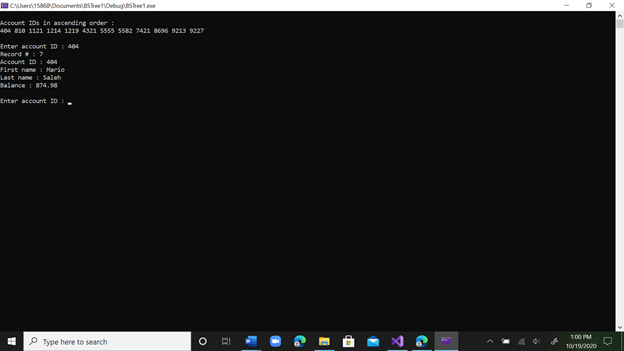
\includegraphics[width=17cm]{Lab9Test2.png}}
\end{DoxyImageNoCaption}



\begin{DoxyImageNoCaption}
  \mbox{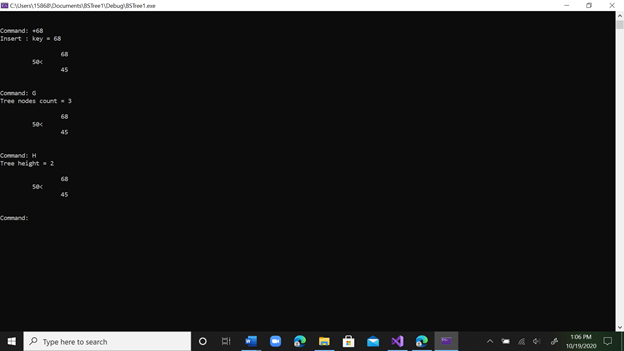
\includegraphics[width=17cm]{Lab9Test3.png}}
\end{DoxyImageNoCaption}



\begin{DoxyImageNoCaption}
  \mbox{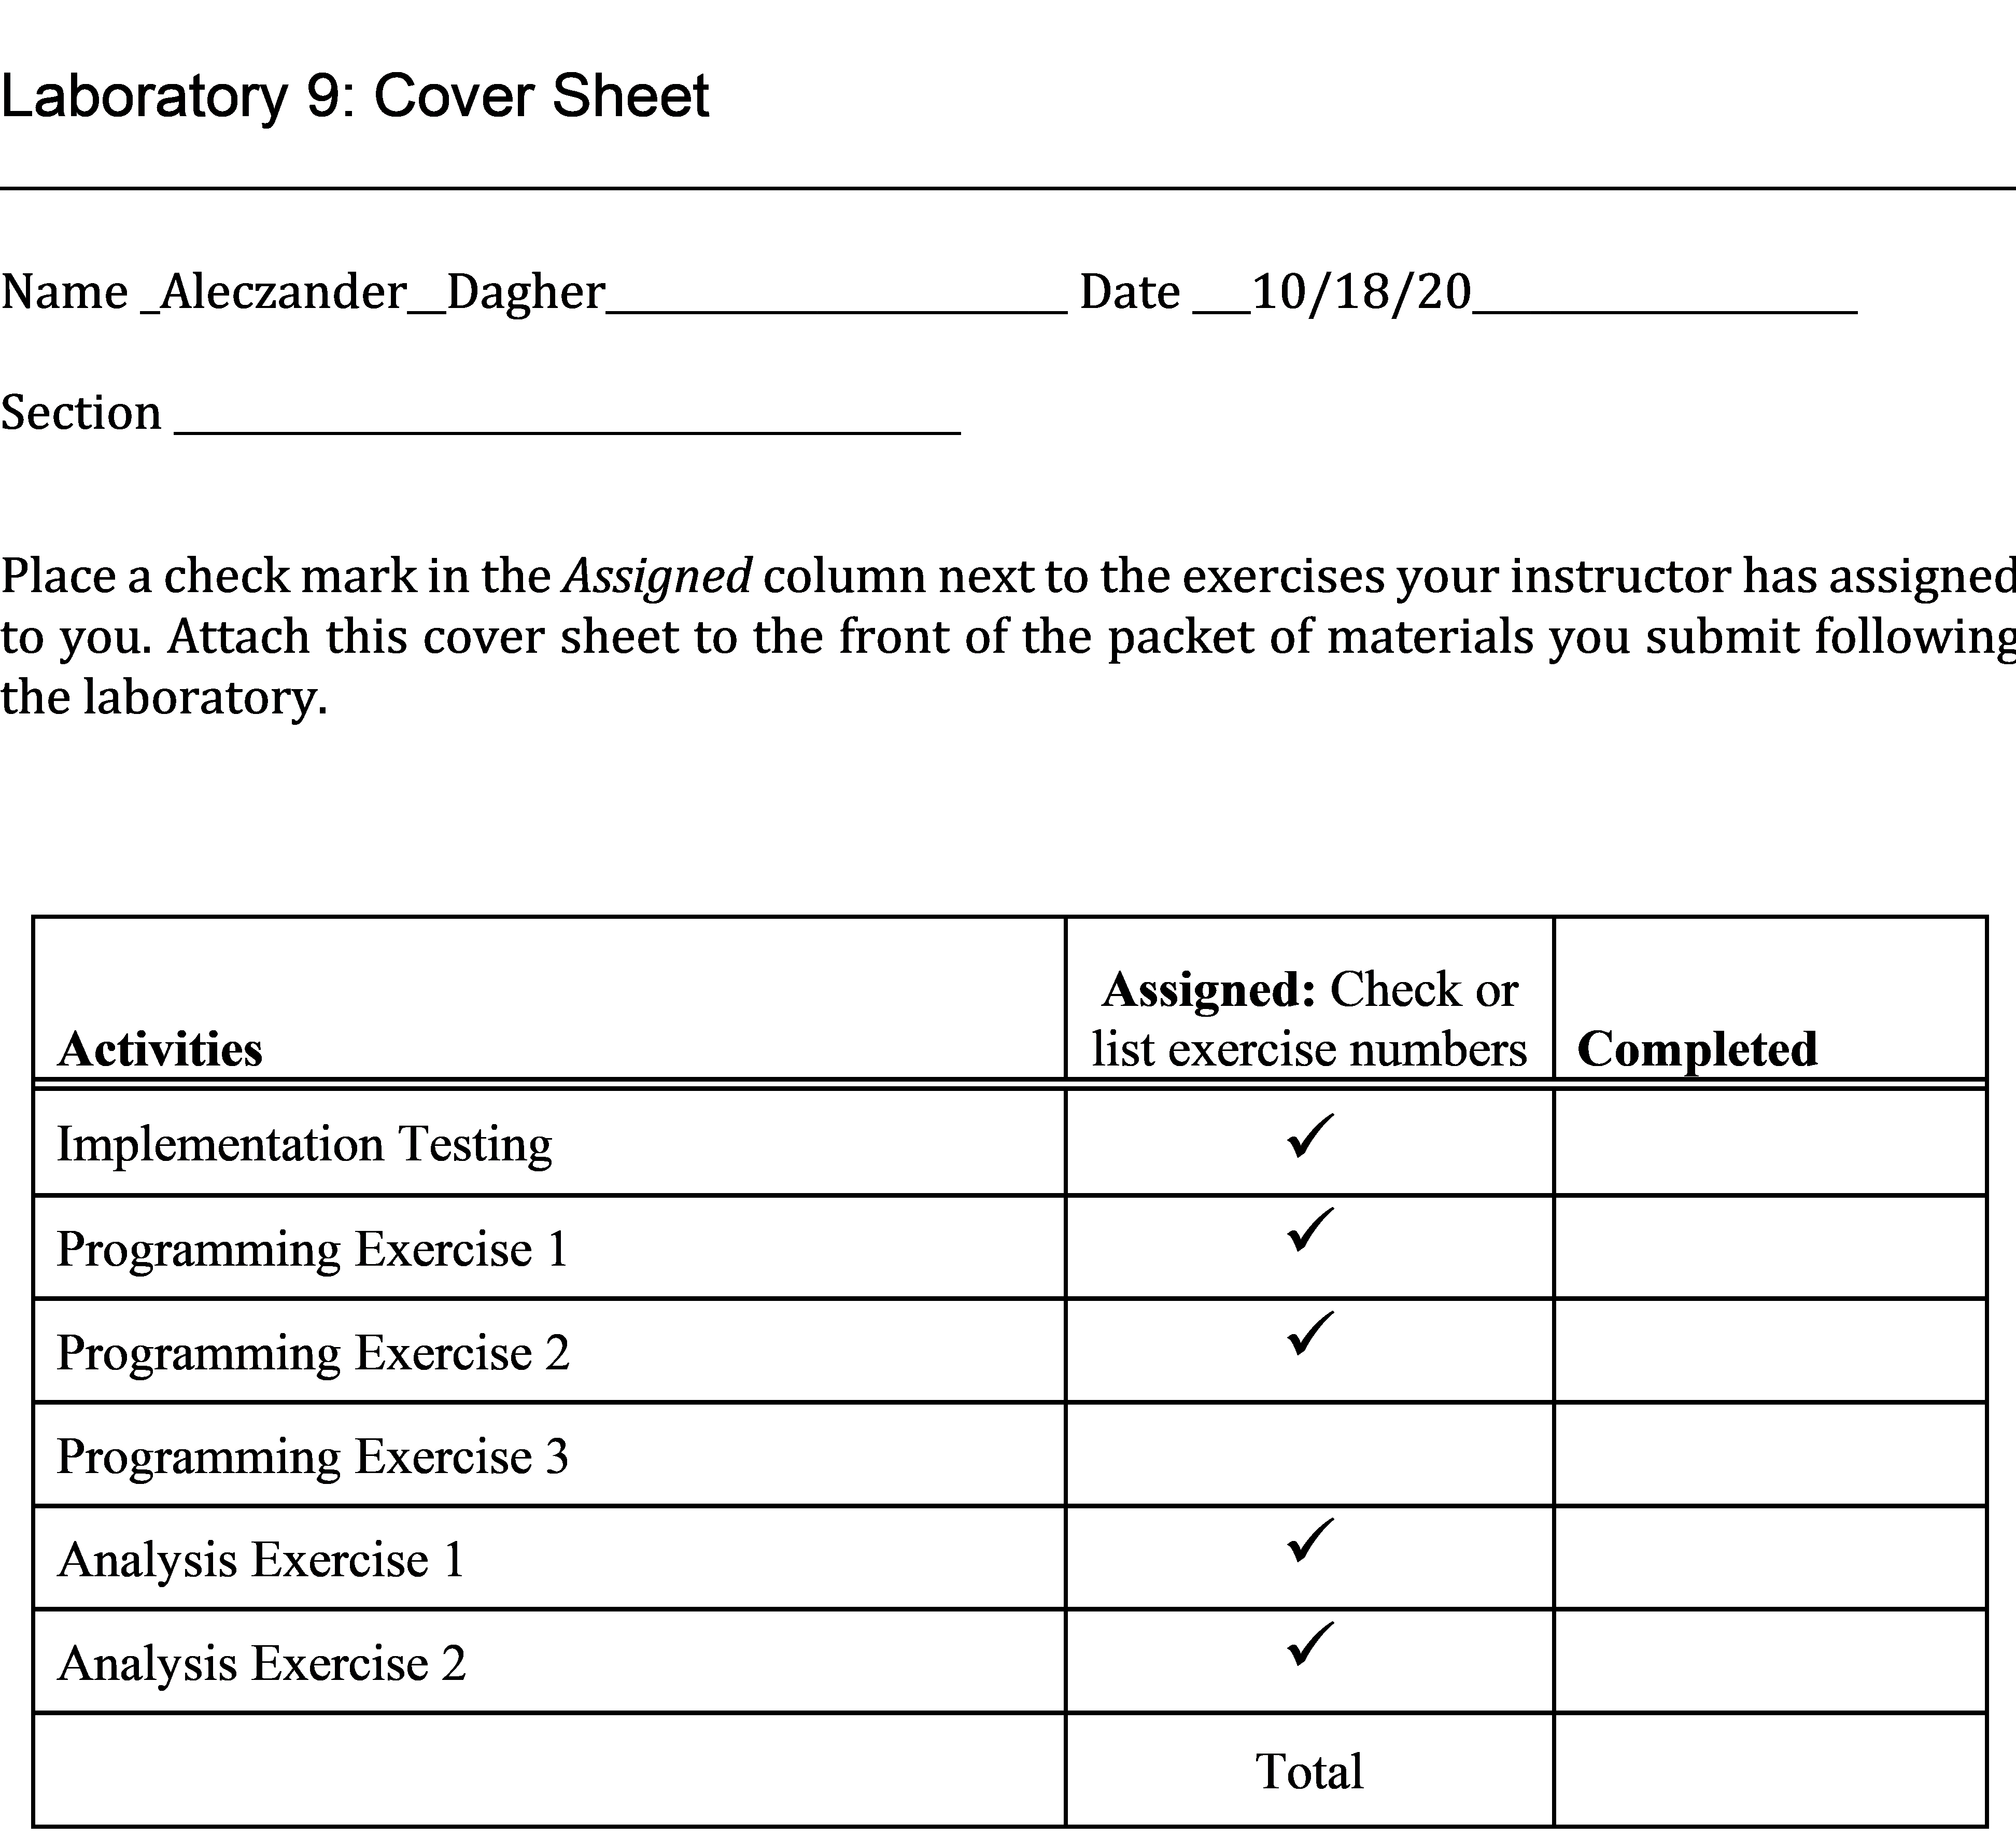
\includegraphics[width=17cm]{Lab9Sheet1.png}}
\end{DoxyImageNoCaption}



\begin{DoxyImageNoCaption}
  \mbox{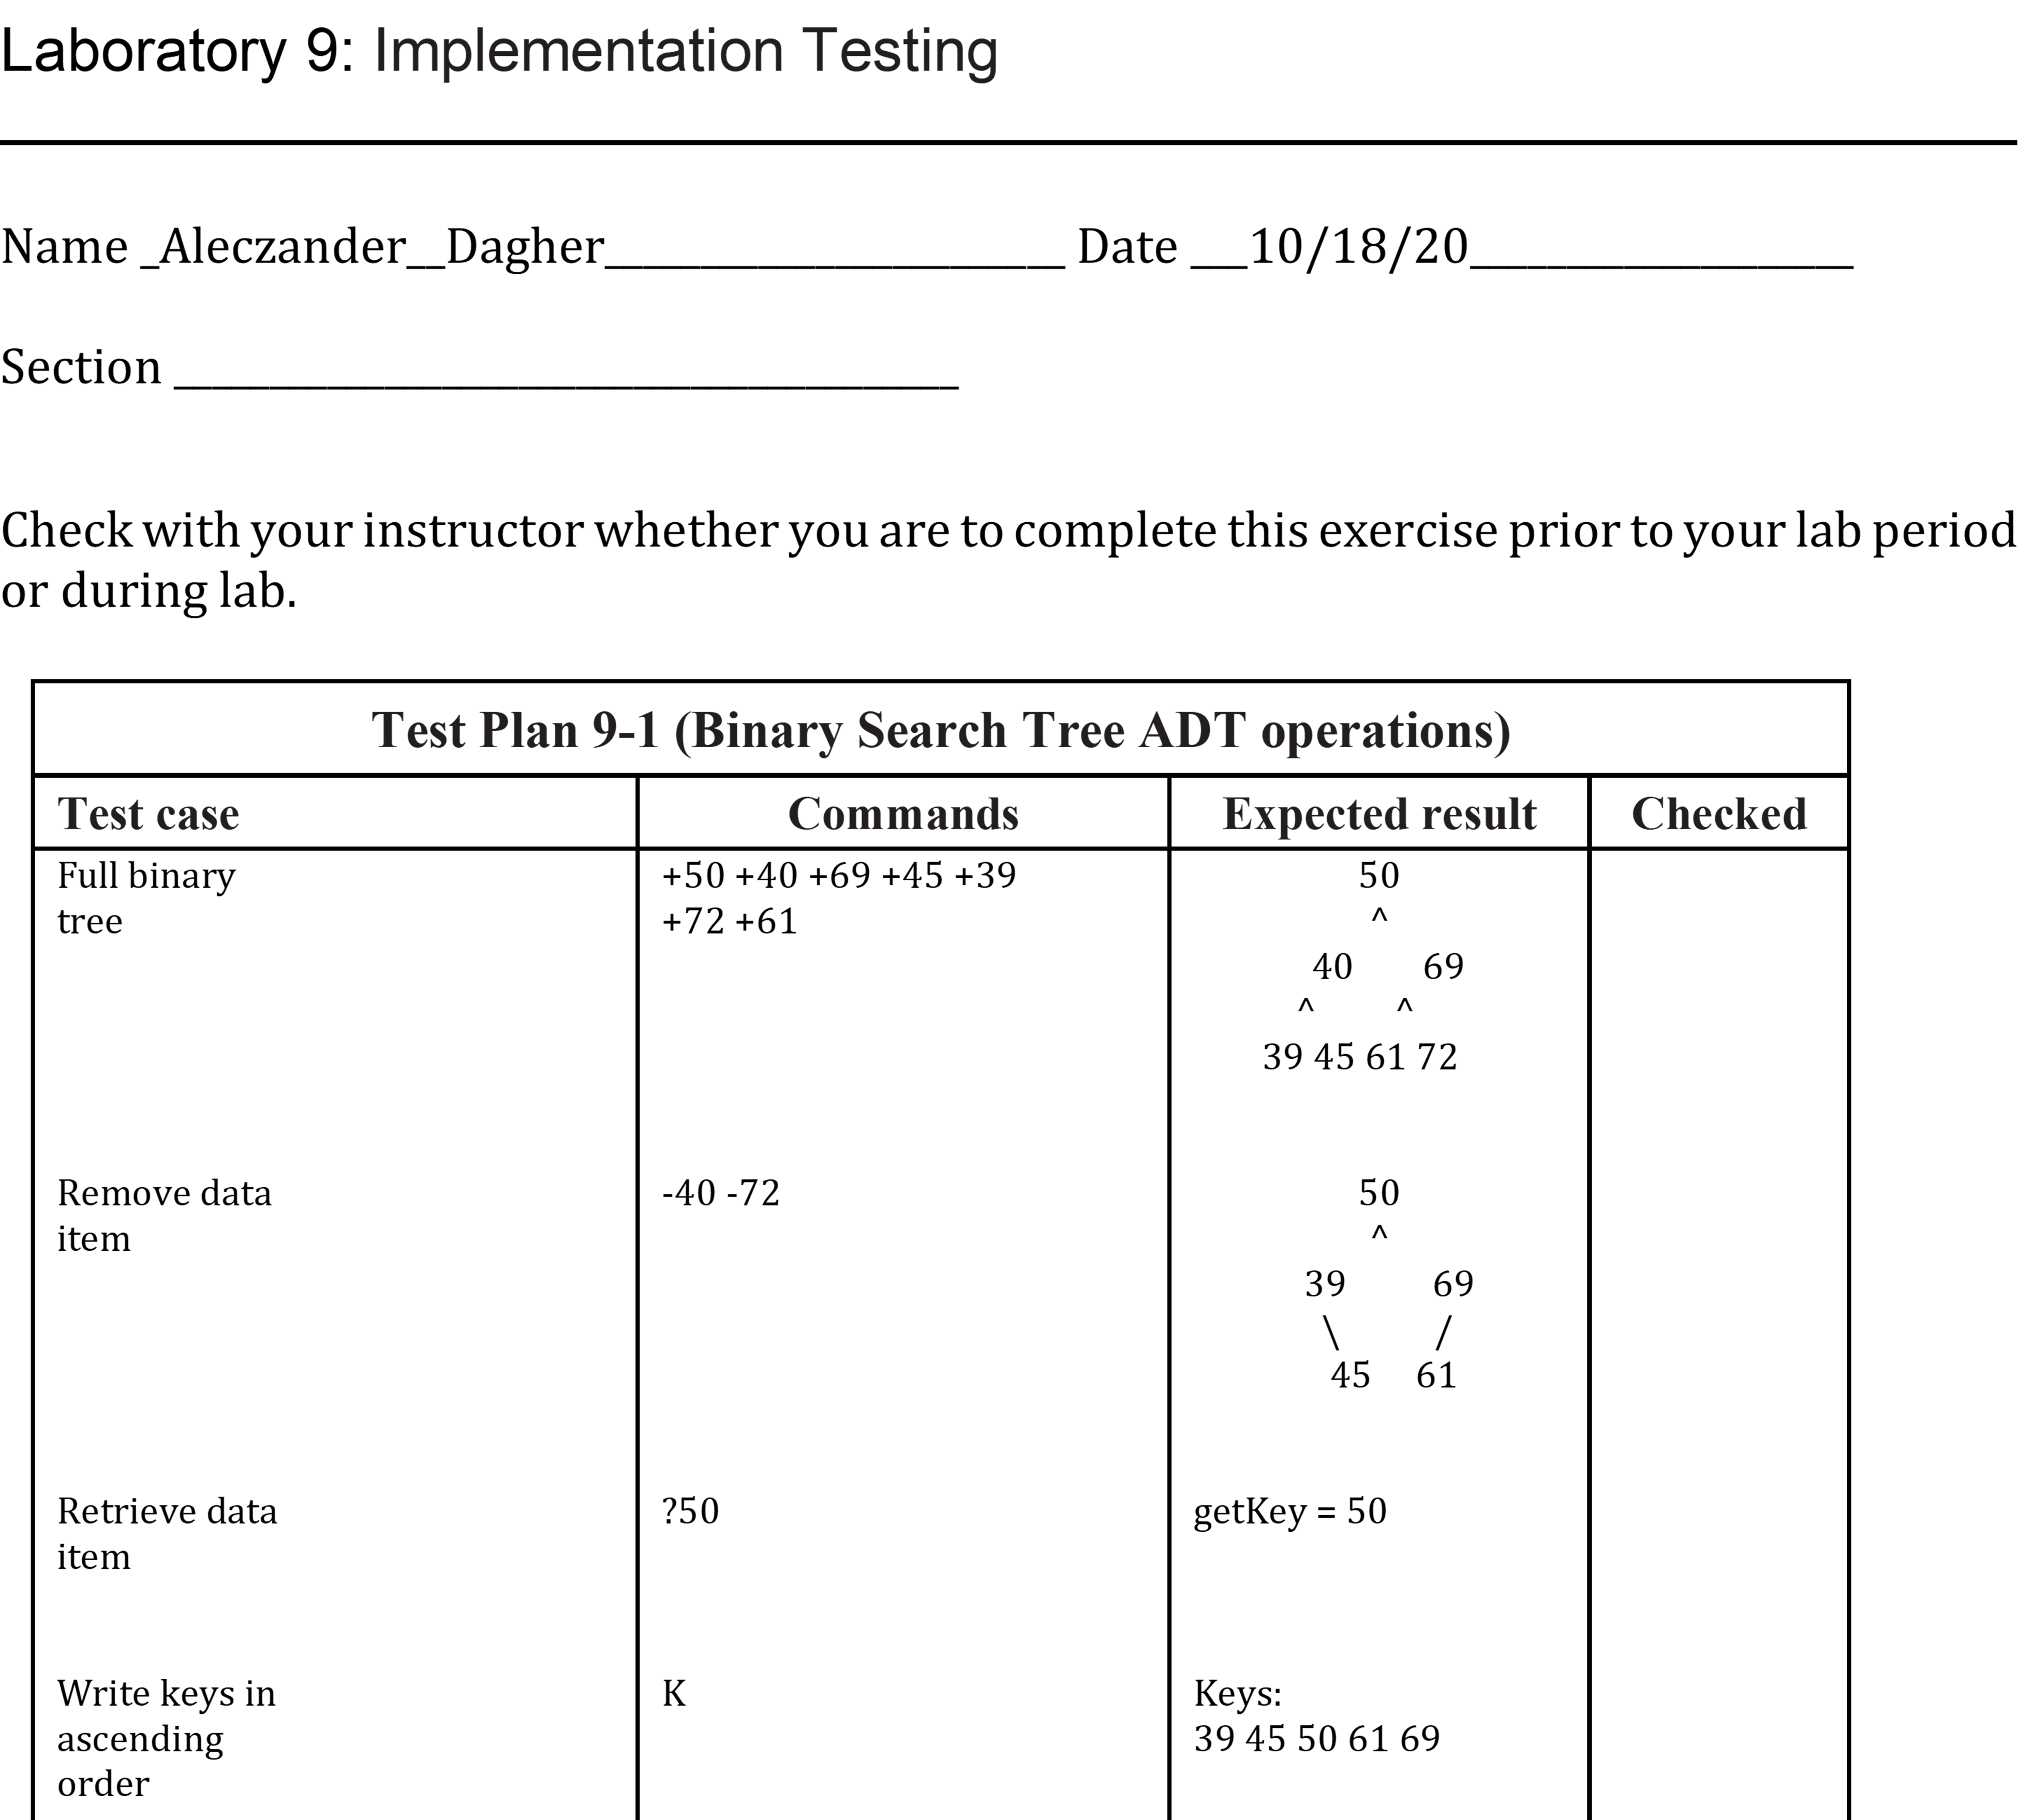
\includegraphics[width=17cm]{Lab9Sheet2.png}}
\end{DoxyImageNoCaption}



\begin{DoxyImageNoCaption}
  \mbox{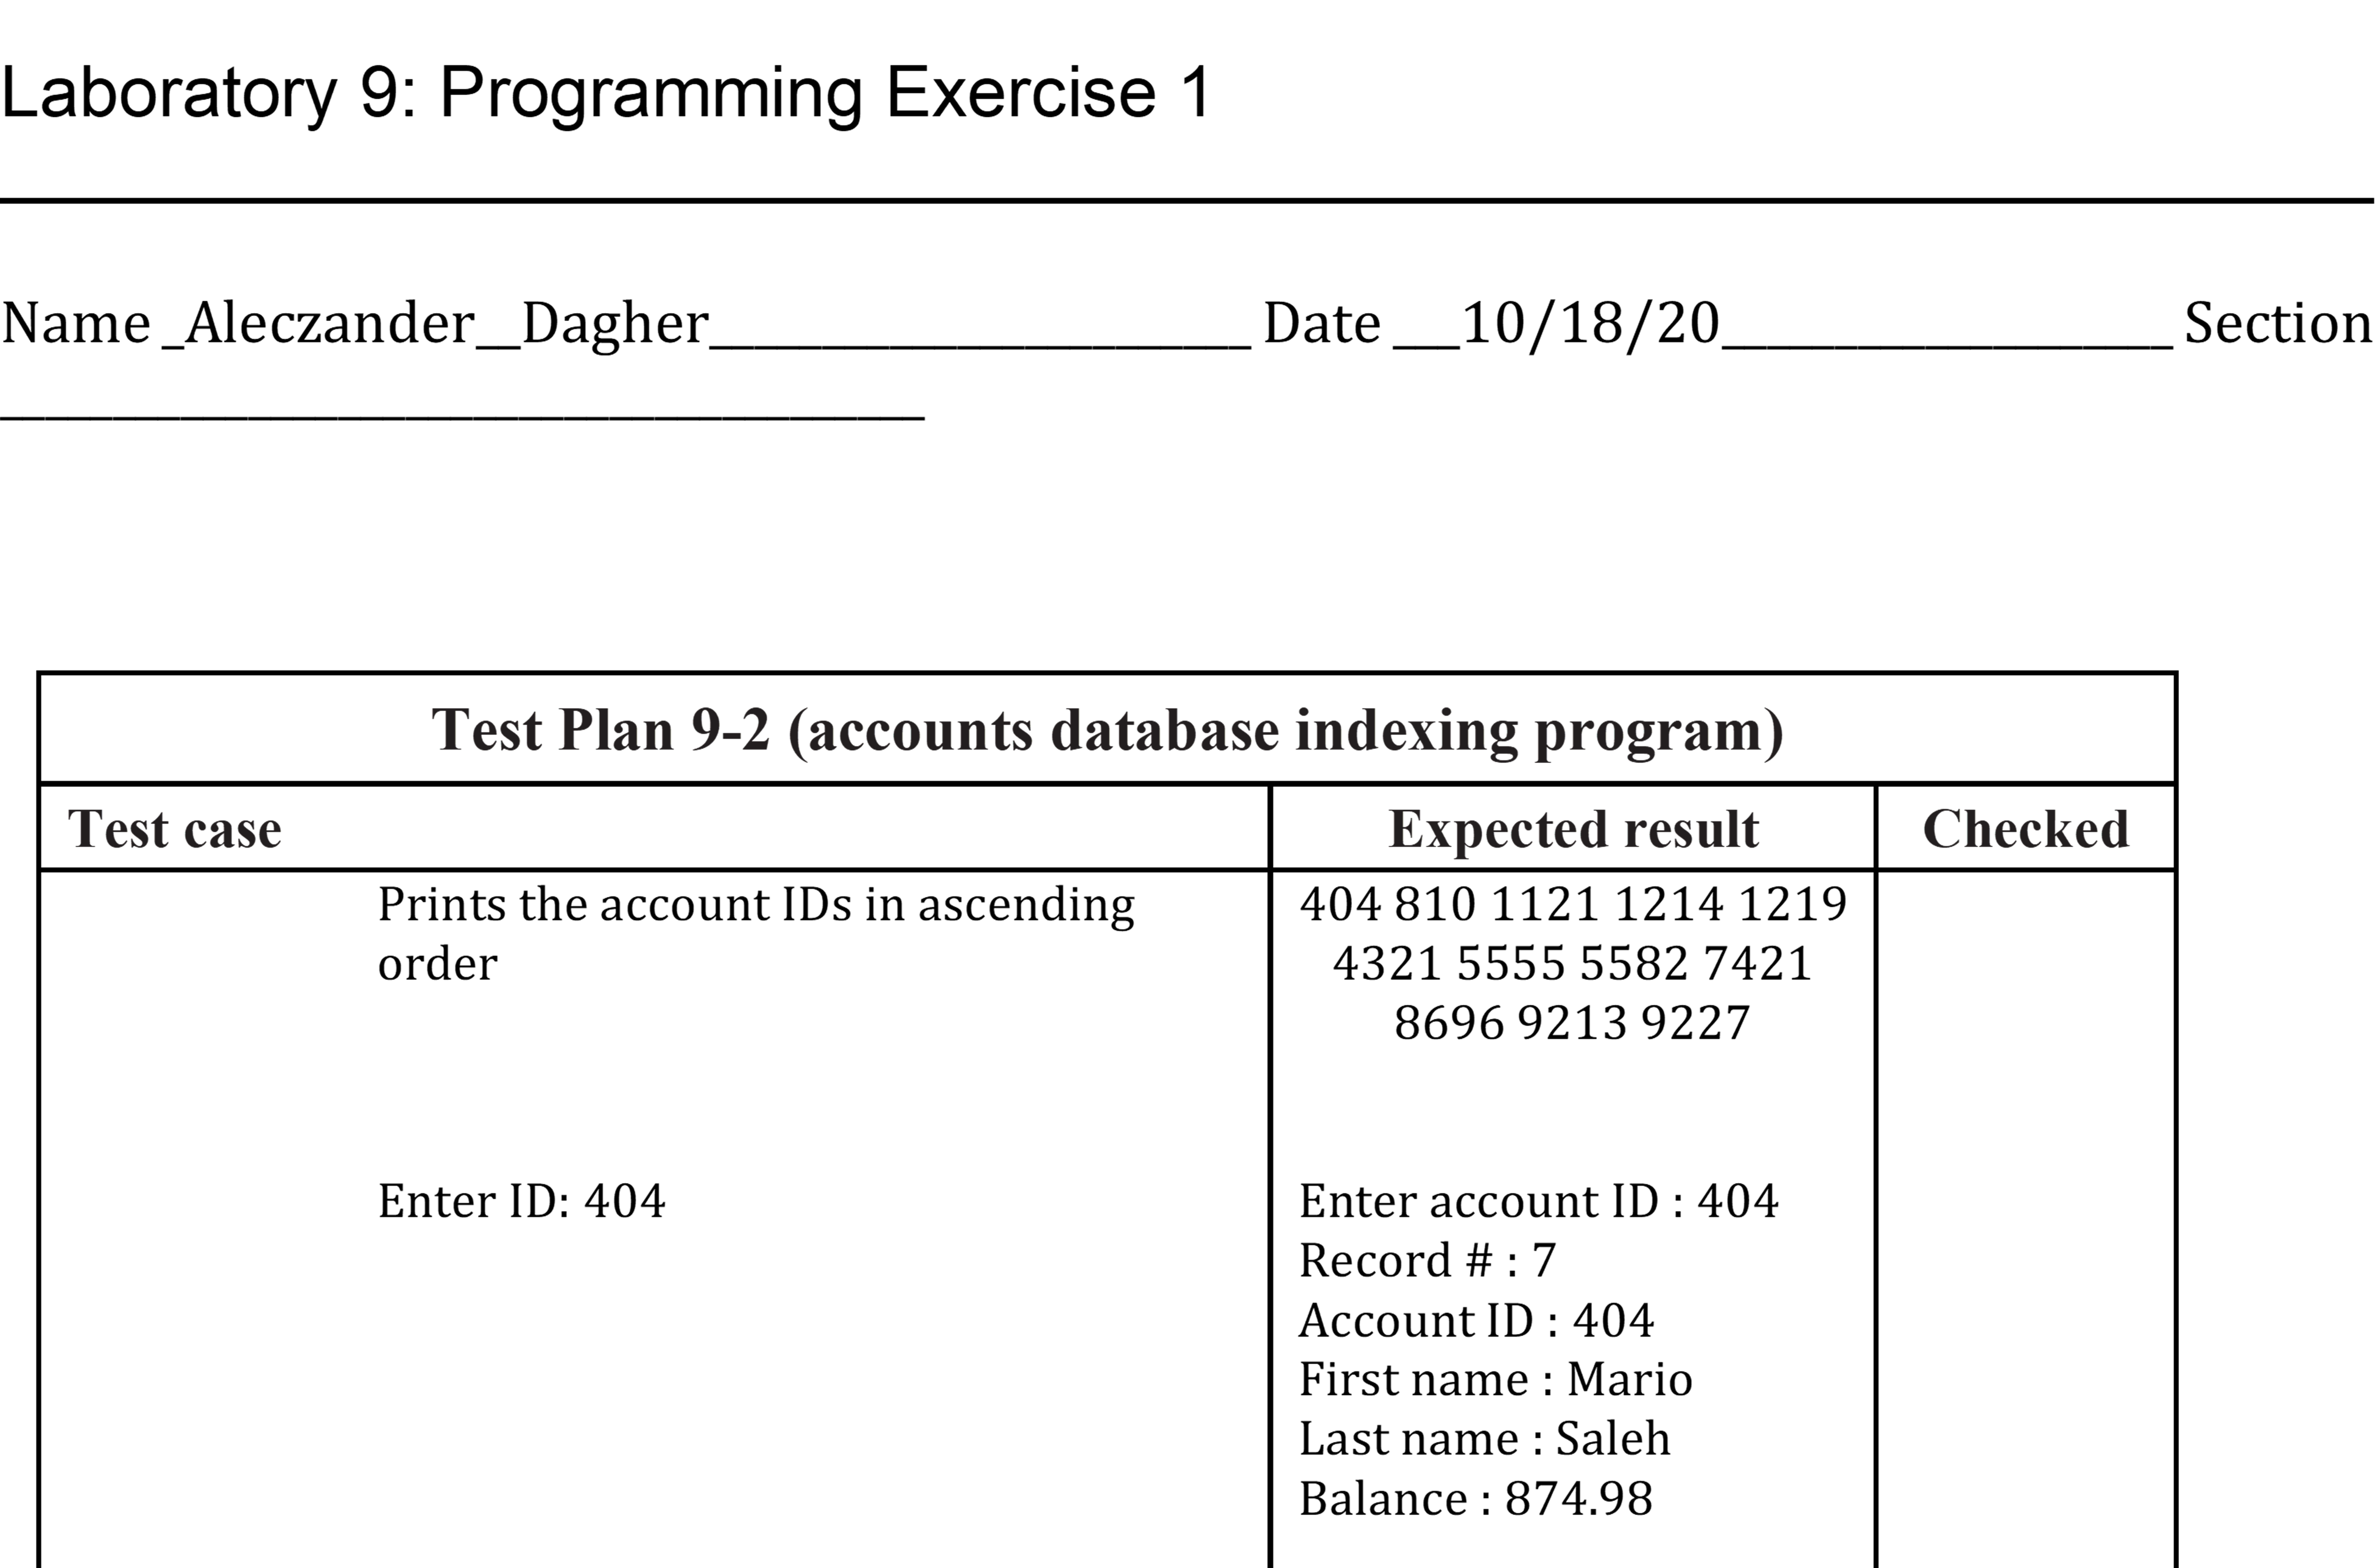
\includegraphics[width=17cm]{Lab9Sheet3.png}}
\end{DoxyImageNoCaption}



\begin{DoxyImageNoCaption}
  \mbox{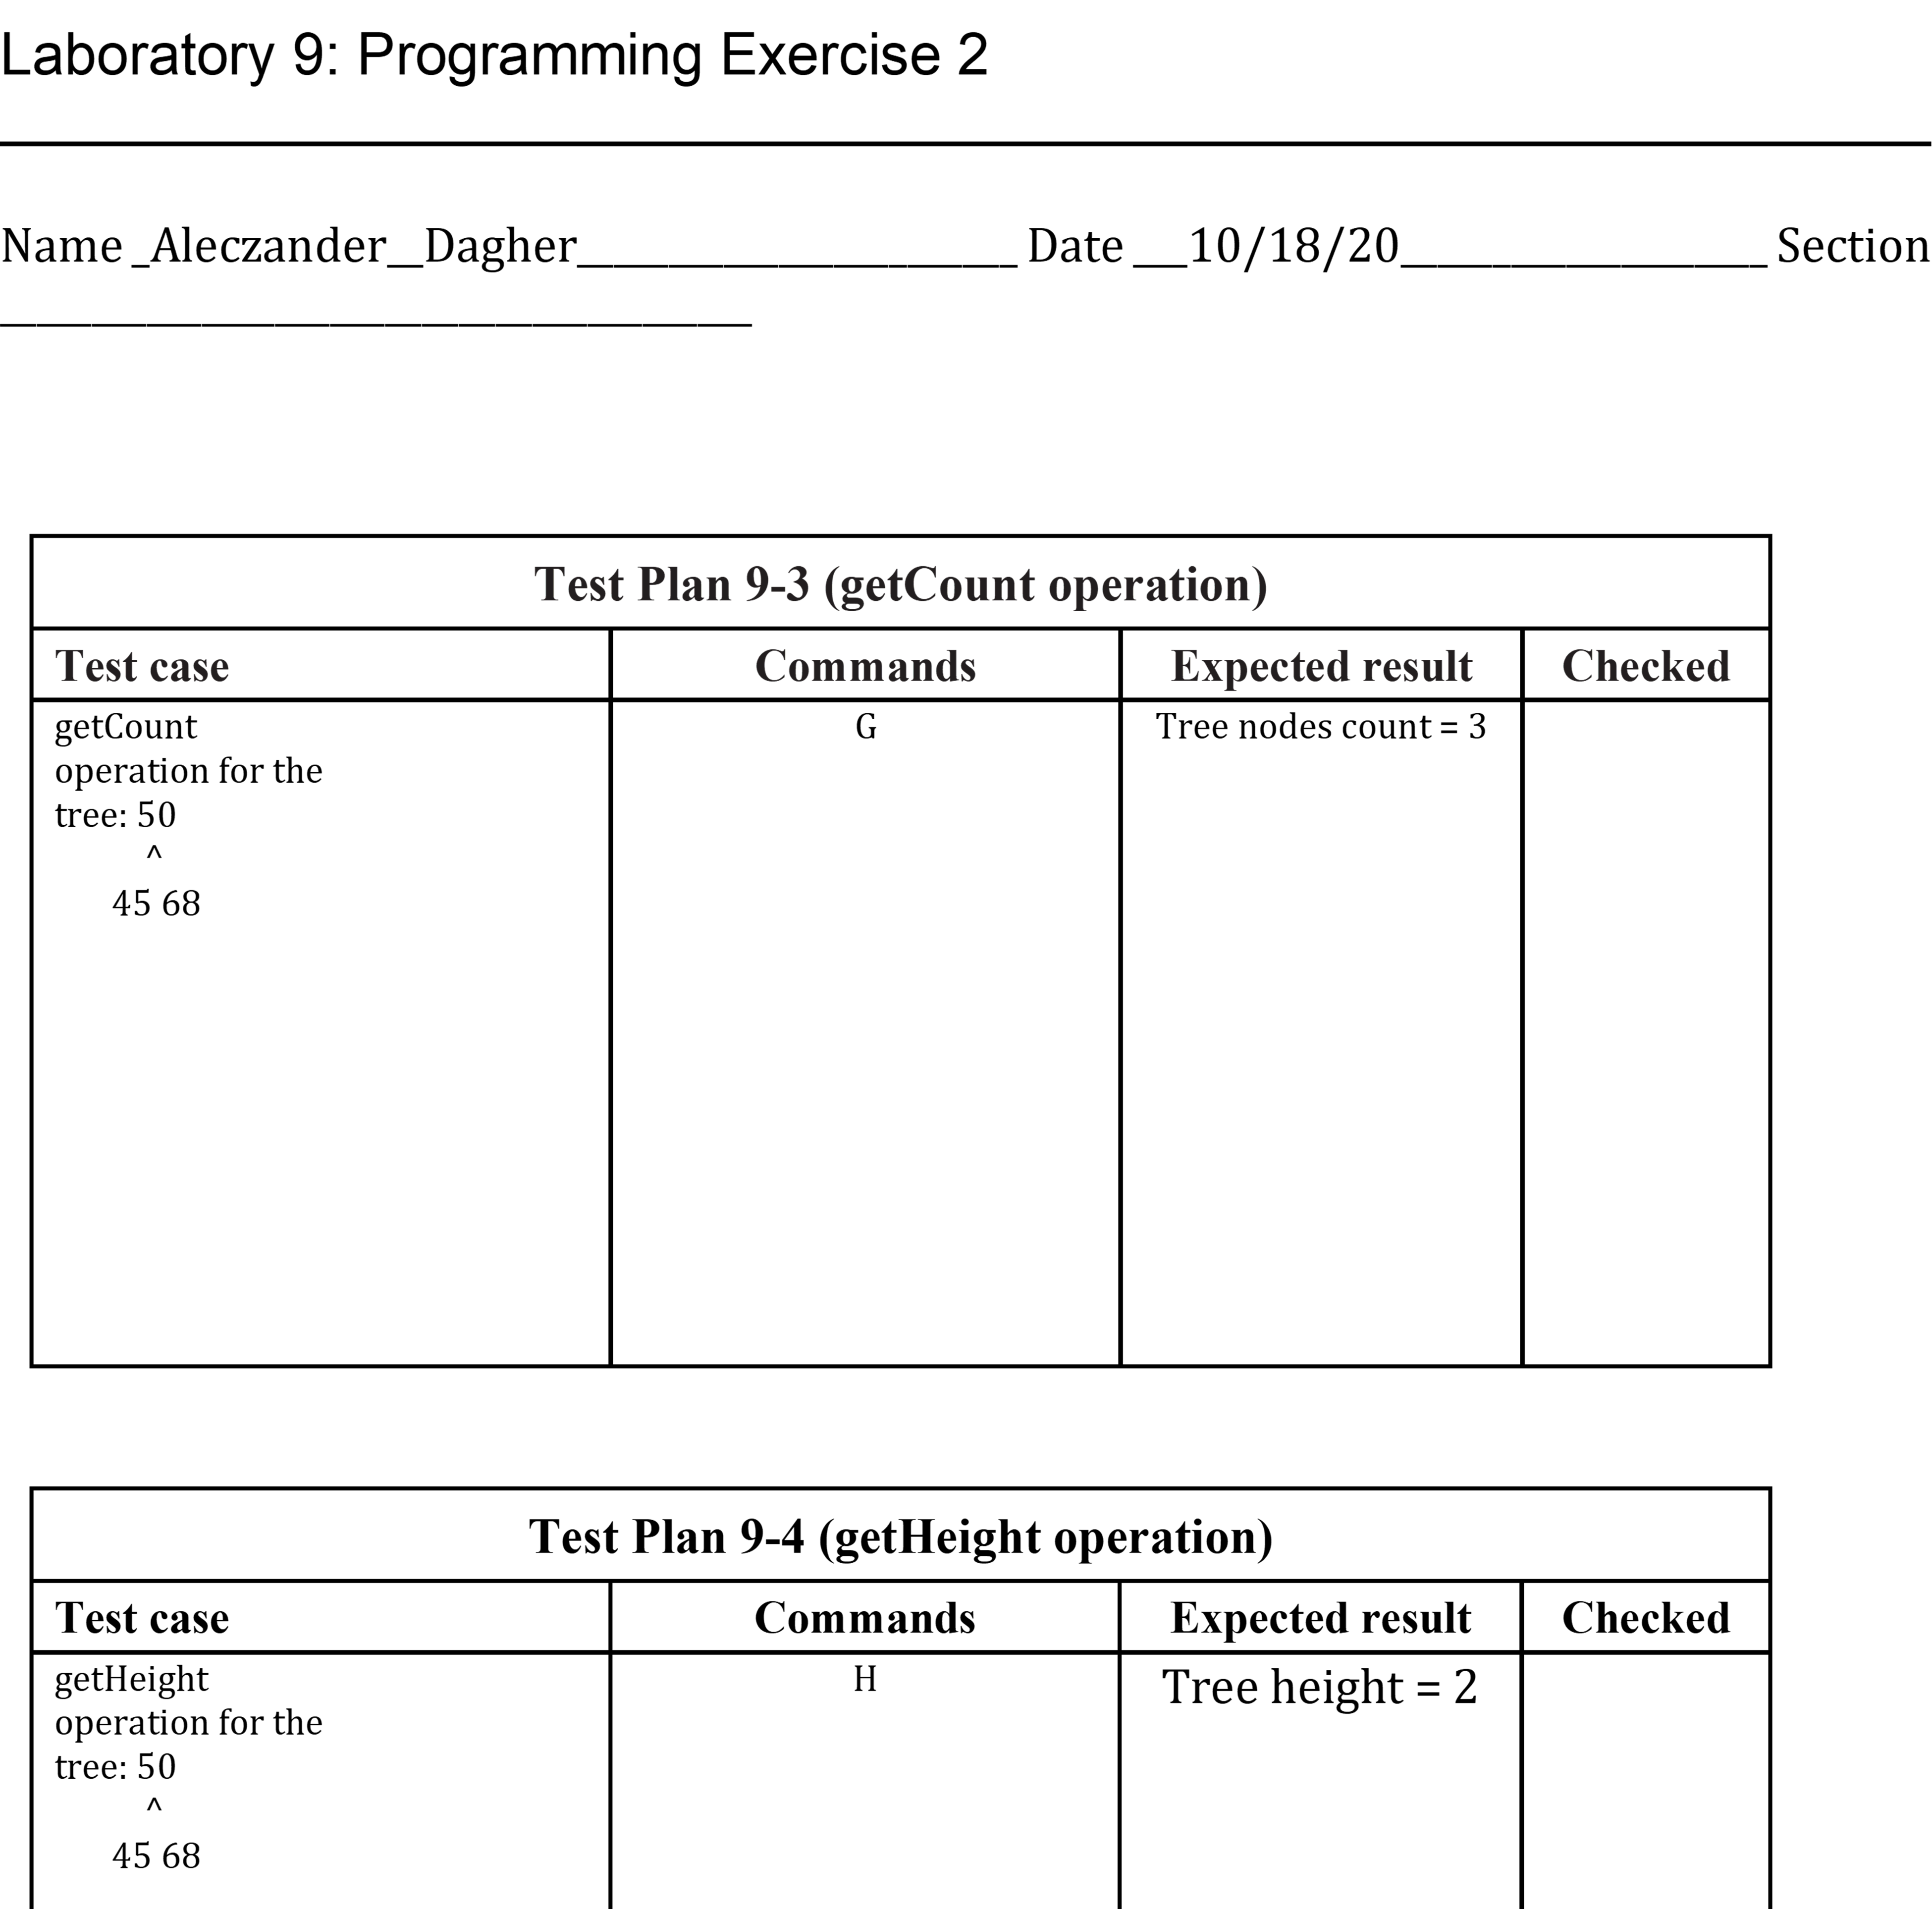
\includegraphics[width=17cm]{Lab9Sheet4.png}}
\end{DoxyImageNoCaption}



\begin{DoxyImageNoCaption}
  \mbox{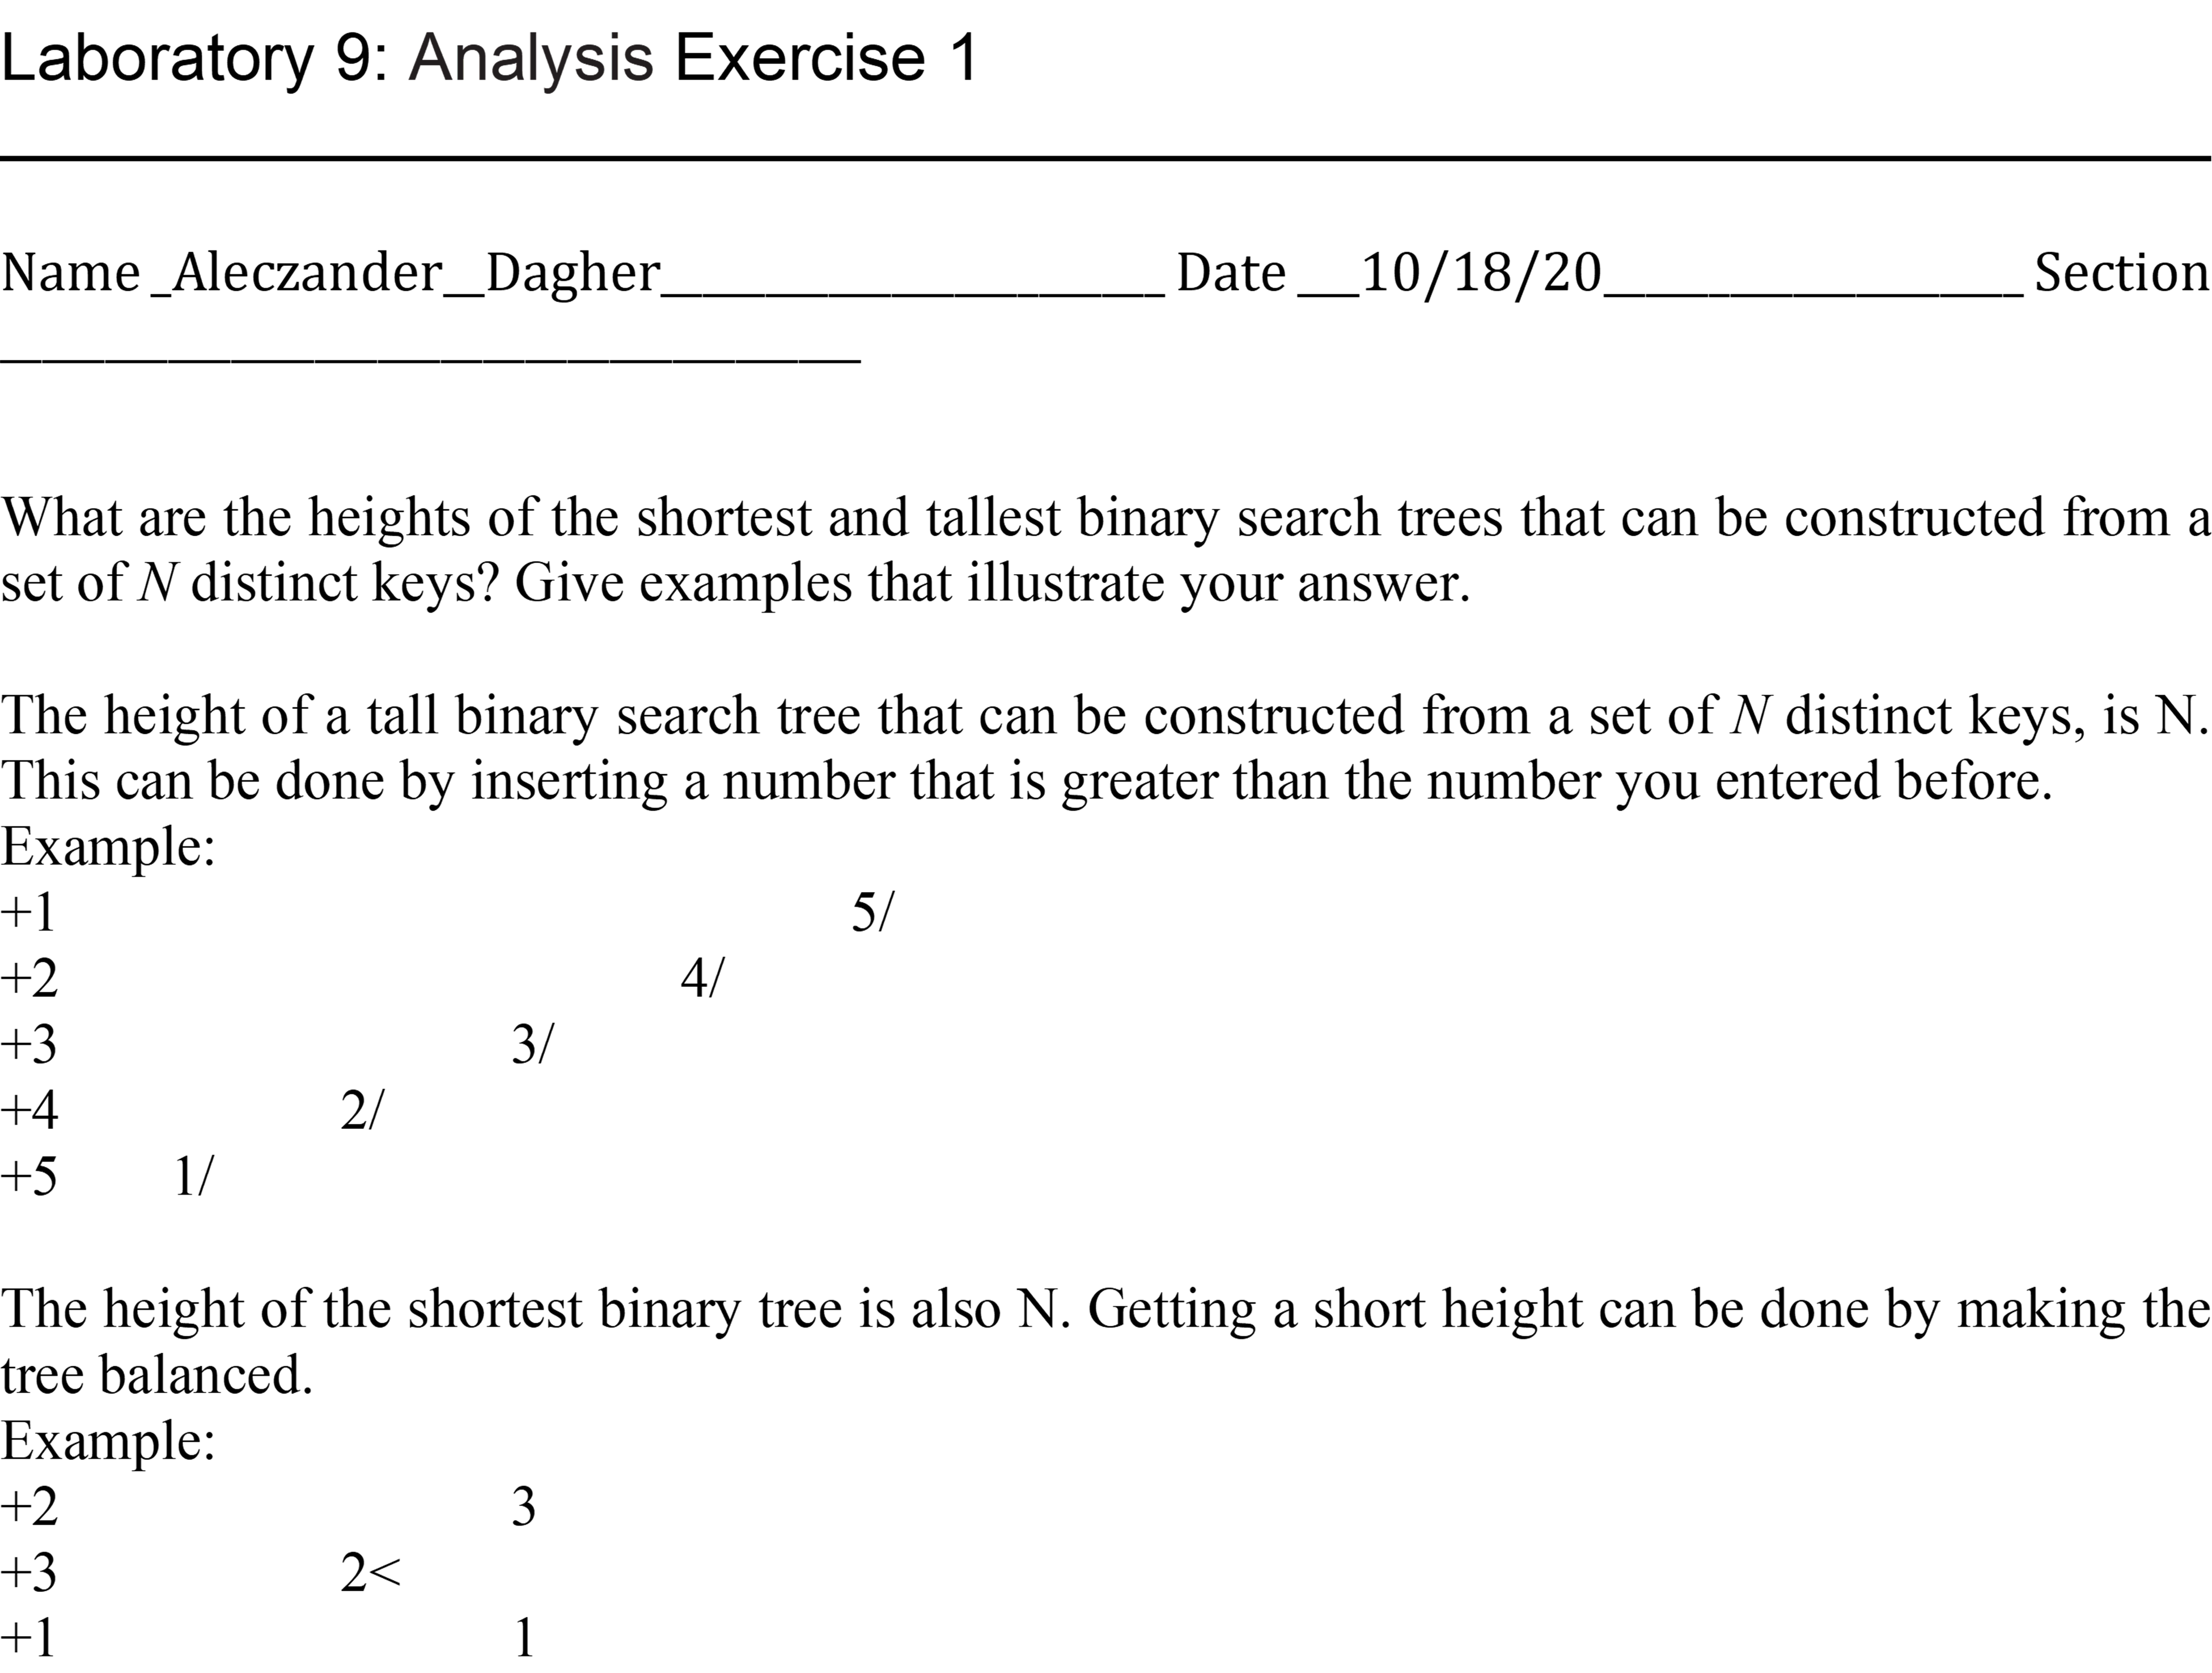
\includegraphics[width=17cm]{Lab9Sheet5.png}}
\end{DoxyImageNoCaption}



\begin{DoxyImageNoCaption}
  \mbox{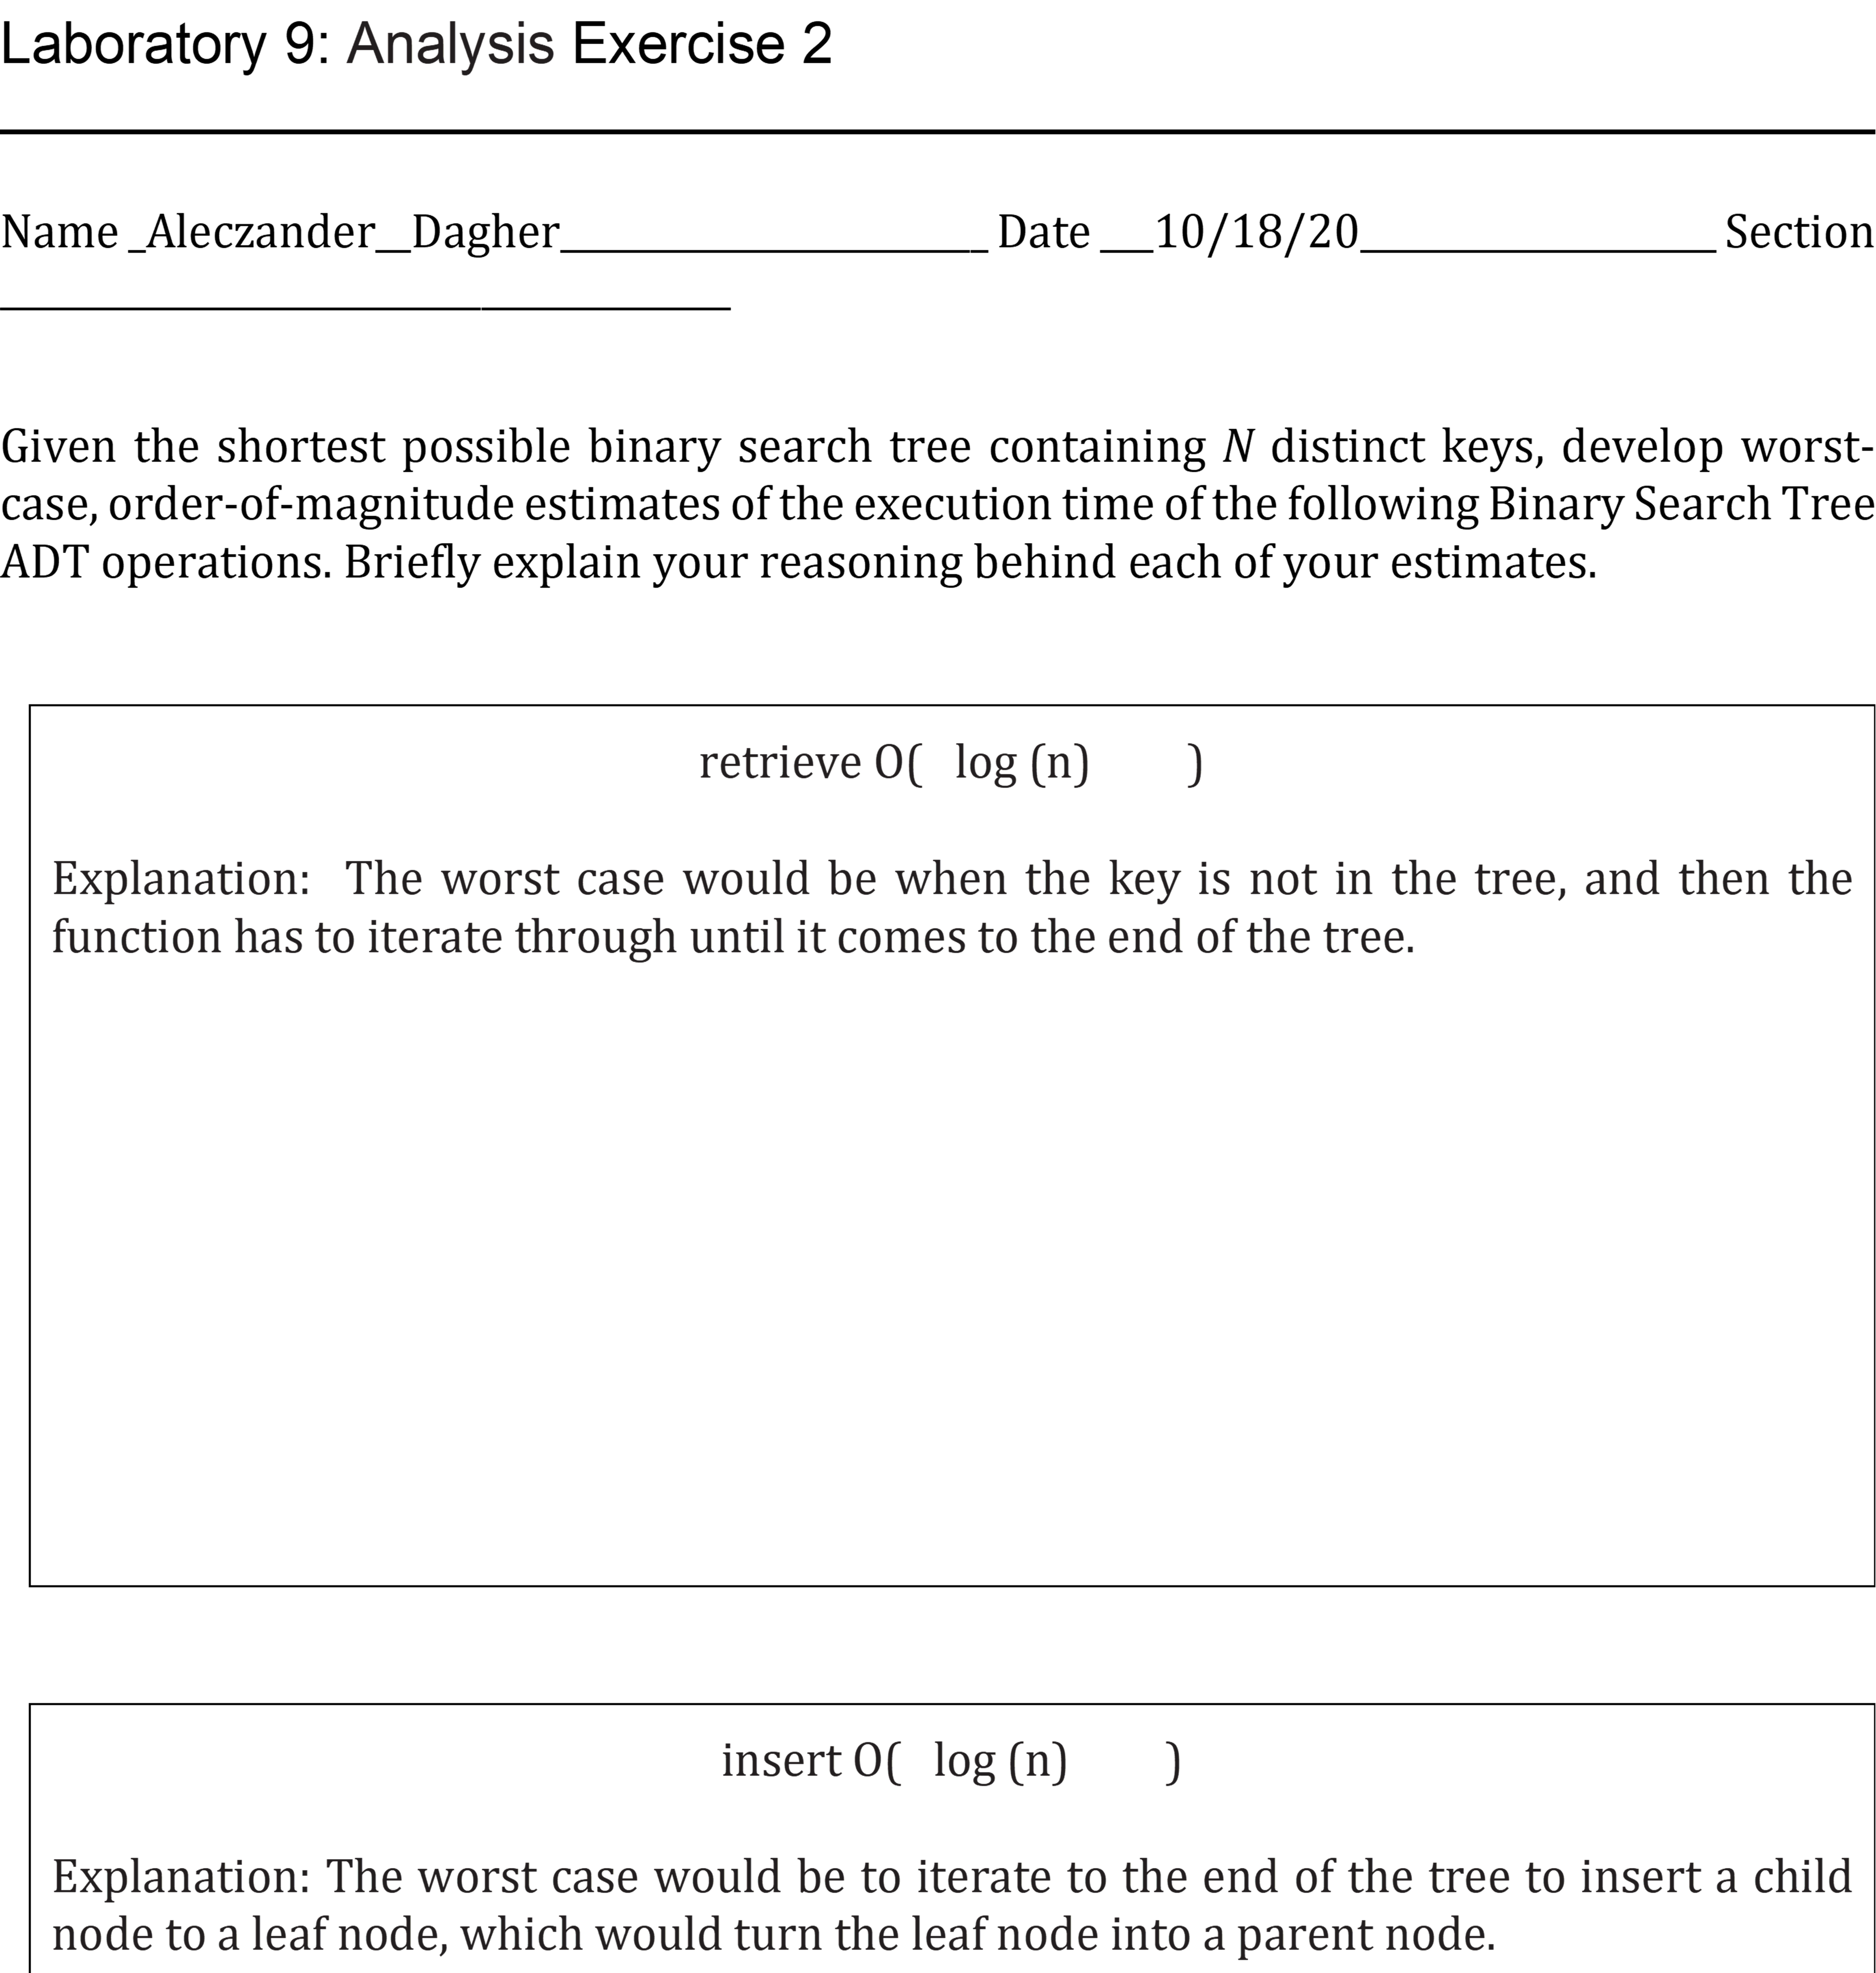
\includegraphics[width=17cm]{Lab9Sheet6.png}}
\end{DoxyImageNoCaption}



\begin{DoxyImageNoCaption}
  \mbox{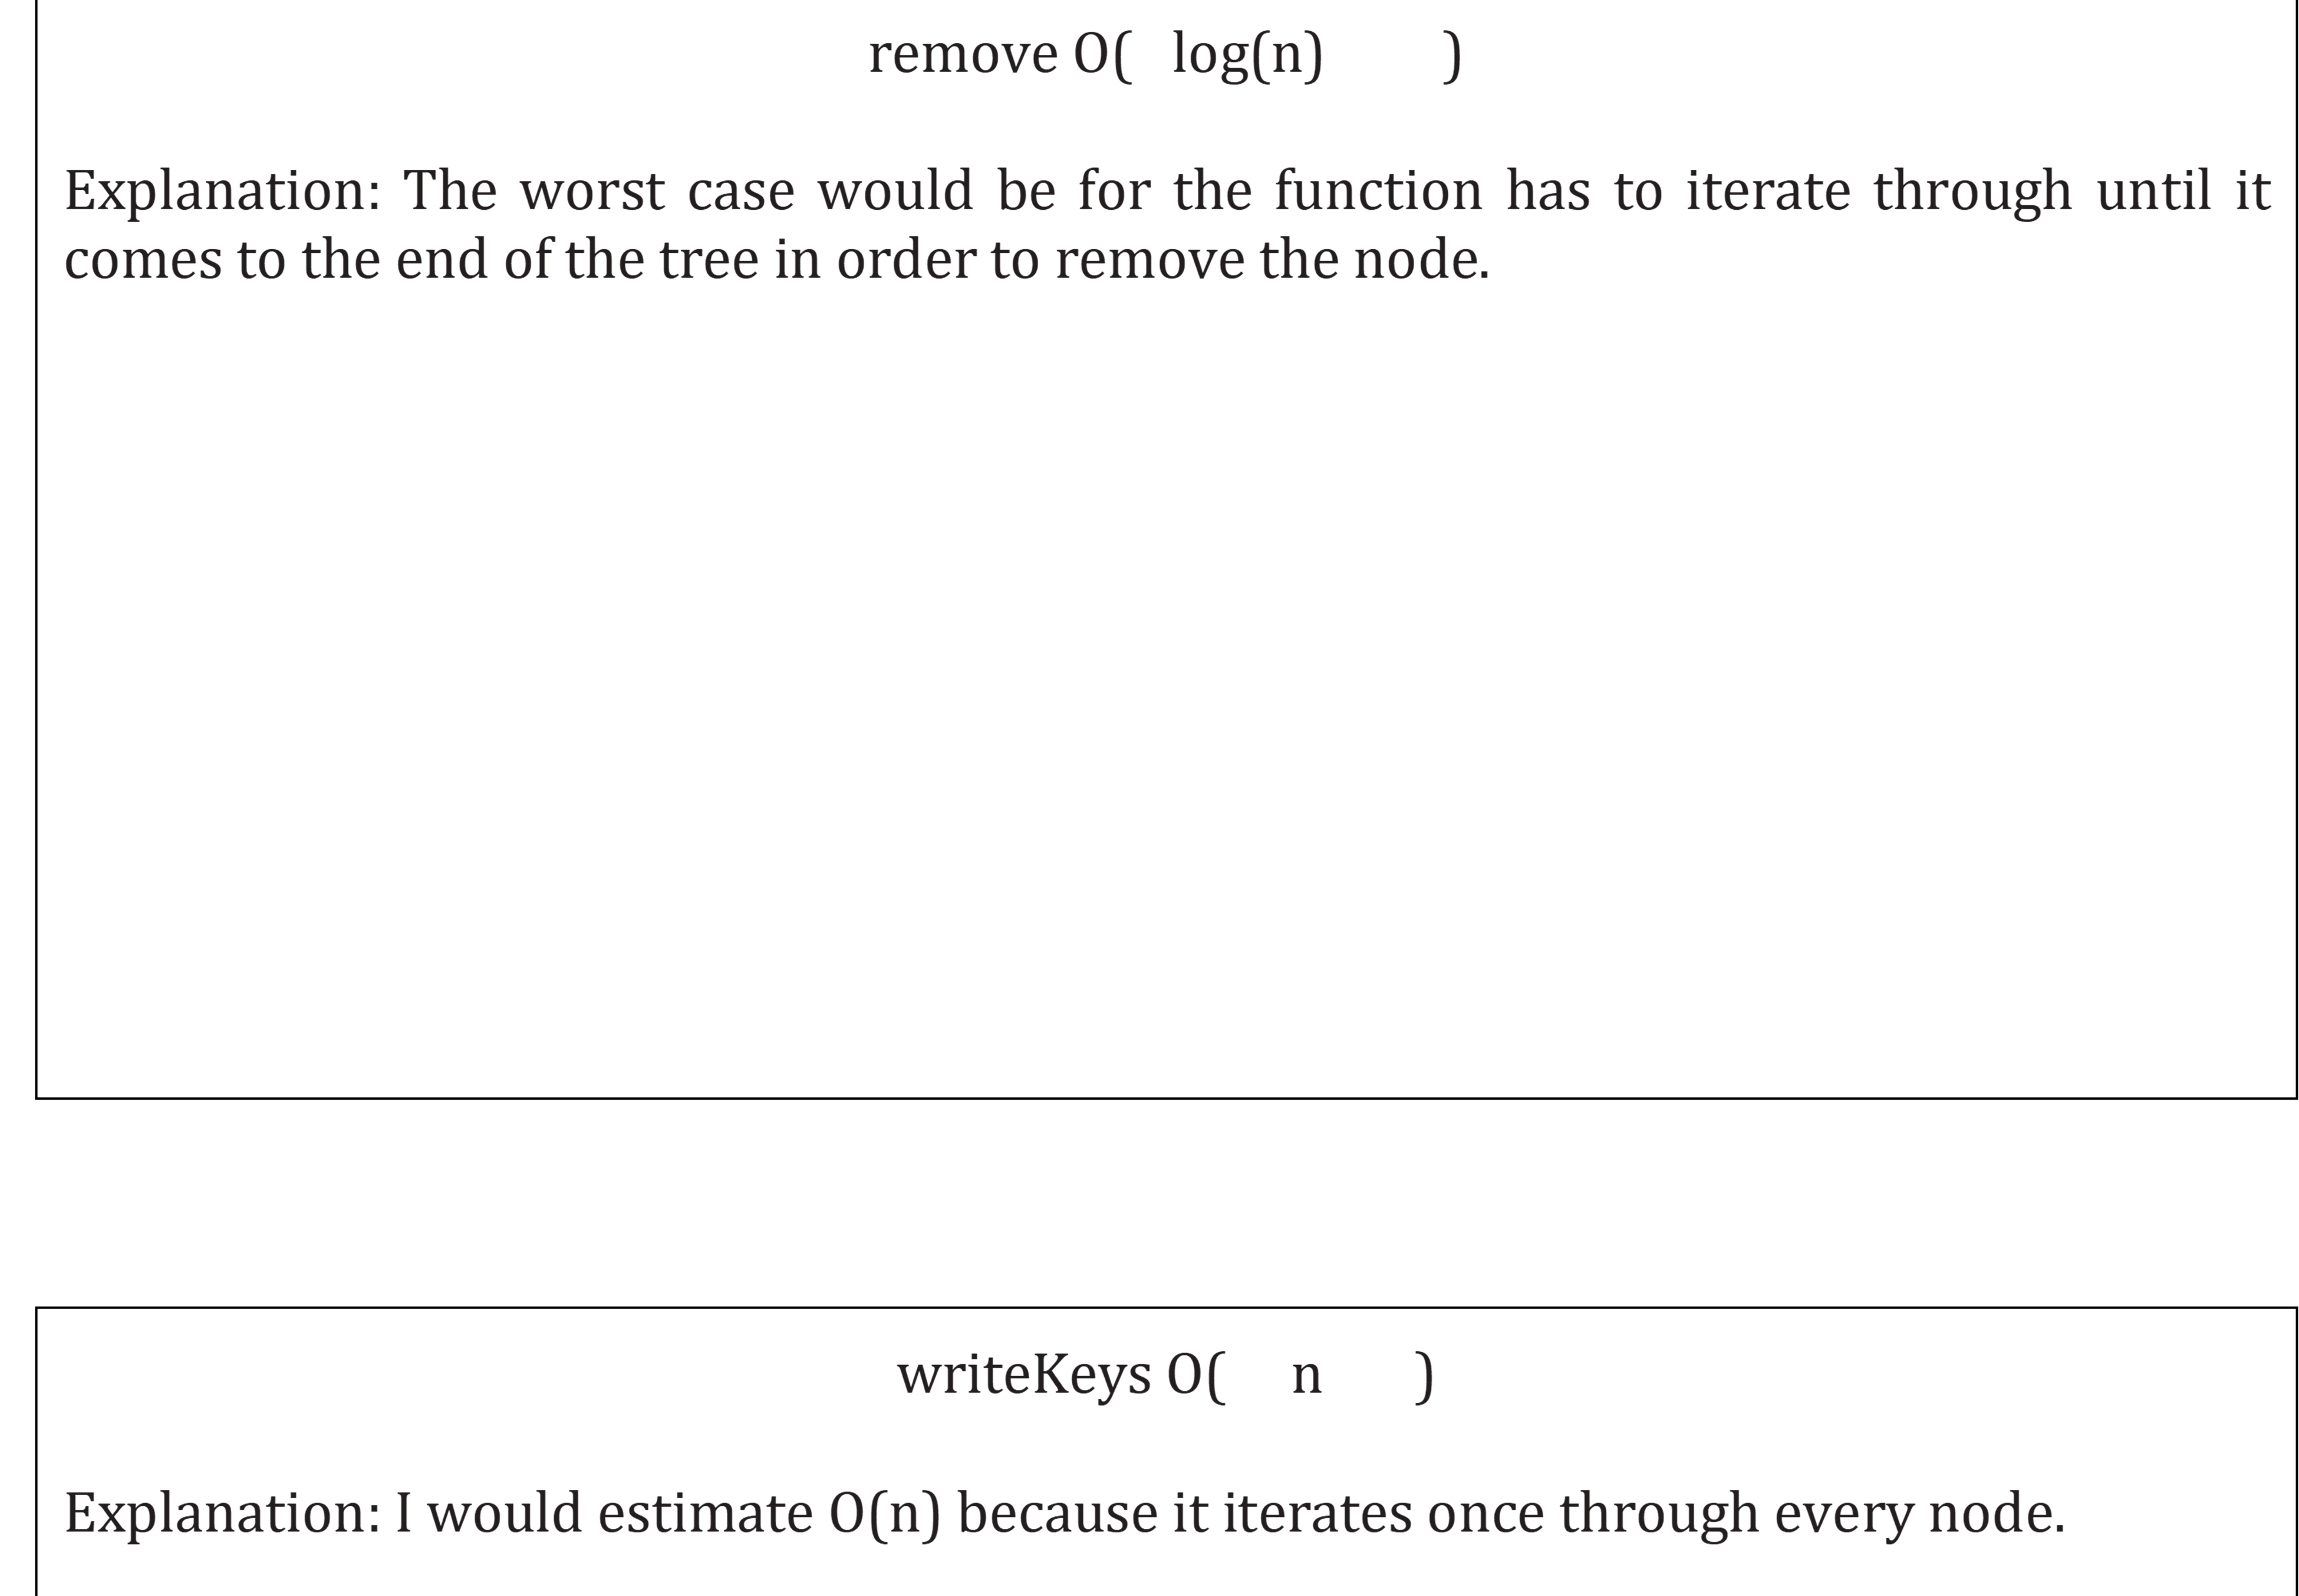
\includegraphics[width=17cm]{Lab9Sheet7.png}}
\end{DoxyImageNoCaption}
 
\chapter{Class Index}
\section{Class List}
Here are the classes, structs, unions and interfaces with brief descriptions\+:\begin{DoxyCompactList}
\item\contentsline{section}{\hyperlink{struct_account_record}{Account\+Record} }{\pageref{struct_account_record}}{}
\item\contentsline{section}{\hyperlink{class_b_s_tree}{B\+S\+Tree$<$ Data\+Type, Key\+Type $>$} }{\pageref{class_b_s_tree}}{}
\item\contentsline{section}{\hyperlink{class_b_s_tree_1_1_b_s_tree_node}{B\+S\+Tree$<$ Data\+Type, Key\+Type $>$\+::\+B\+S\+Tree\+Node} }{\pageref{class_b_s_tree_1_1_b_s_tree_node}}{}
\item\contentsline{section}{\hyperlink{struct_index_entry}{Index\+Entry} }{\pageref{struct_index_entry}}{}
\end{DoxyCompactList}

\chapter{File Index}
\section{File List}
Here is a list of all files with brief descriptions\+:\begin{DoxyCompactList}
\item\contentsline{section}{\hyperlink{_b_s_tree_8cpp}{B\+S\+Tree.\+cpp} }{\pageref{_b_s_tree_8cpp}}{}
\item\contentsline{section}{\hyperlink{_b_s_tree_8h}{B\+S\+Tree.\+h} }{\pageref{_b_s_tree_8h}}{}
\item\contentsline{section}{\hyperlink{database_8cpp}{database.\+cpp} }{\pageref{database_8cpp}}{}
\end{DoxyCompactList}

\chapter{Class Documentation}
\hypertarget{struct_account_record}{}\section{Account\+Record Struct Reference}
\label{struct_account_record}\index{Account\+Record@{Account\+Record}}
\subsection*{Public Attributes}
\begin{DoxyCompactItemize}
\item 
int \hyperlink{struct_account_record_a587aa92adcd387d37427cd19c69e5932}{acct\+ID}
\item 
char \hyperlink{struct_account_record_a89df48cc152b78efda9060a0cc461dd1}{first\+Name} \mbox{[}\hyperlink{database_8cpp_a5d9687231dabb10b55cd7598e1be6702}{name\+Length}\mbox{]}
\item 
char \hyperlink{struct_account_record_ab9b4c37852573096dd9c81bec70f68b9}{last\+Name} \mbox{[}\hyperlink{database_8cpp_a5d9687231dabb10b55cd7598e1be6702}{name\+Length}\mbox{]}
\item 
double \hyperlink{struct_account_record_a7de857c68a45702a0c1c4720b4570c2a}{balance}
\end{DoxyCompactItemize}


\subsection{Member Data Documentation}
\hypertarget{struct_account_record_a587aa92adcd387d37427cd19c69e5932}{}\label{struct_account_record_a587aa92adcd387d37427cd19c69e5932} 
\index{Account\+Record@{Account\+Record}!acct\+ID@{acct\+ID}}
\index{acct\+ID@{acct\+ID}!Account\+Record@{Account\+Record}}
\subsubsection{\texorpdfstring{acct\+ID}{acctID}}
{\footnotesize\ttfamily int Account\+Record\+::acct\+ID}

\hypertarget{struct_account_record_a7de857c68a45702a0c1c4720b4570c2a}{}\label{struct_account_record_a7de857c68a45702a0c1c4720b4570c2a} 
\index{Account\+Record@{Account\+Record}!balance@{balance}}
\index{balance@{balance}!Account\+Record@{Account\+Record}}
\subsubsection{\texorpdfstring{balance}{balance}}
{\footnotesize\ttfamily double Account\+Record\+::balance}

\hypertarget{struct_account_record_a89df48cc152b78efda9060a0cc461dd1}{}\label{struct_account_record_a89df48cc152b78efda9060a0cc461dd1} 
\index{Account\+Record@{Account\+Record}!first\+Name@{first\+Name}}
\index{first\+Name@{first\+Name}!Account\+Record@{Account\+Record}}
\subsubsection{\texorpdfstring{first\+Name}{firstName}}
{\footnotesize\ttfamily char Account\+Record\+::first\+Name\mbox{[}\hyperlink{database_8cpp_a5d9687231dabb10b55cd7598e1be6702}{name\+Length}\mbox{]}}

\hypertarget{struct_account_record_ab9b4c37852573096dd9c81bec70f68b9}{}\label{struct_account_record_ab9b4c37852573096dd9c81bec70f68b9} 
\index{Account\+Record@{Account\+Record}!last\+Name@{last\+Name}}
\index{last\+Name@{last\+Name}!Account\+Record@{Account\+Record}}
\subsubsection{\texorpdfstring{last\+Name}{lastName}}
{\footnotesize\ttfamily char Account\+Record\+::last\+Name\mbox{[}\hyperlink{database_8cpp_a5d9687231dabb10b55cd7598e1be6702}{name\+Length}\mbox{]}}



The documentation for this struct was generated from the following file\+:\begin{DoxyCompactItemize}
\item 
\hyperlink{database_8cpp}{database.\+cpp}\end{DoxyCompactItemize}

\hypertarget{class_b_s_tree}{}\section{B\+S\+Tree$<$ Data\+Type, Key\+Type $>$ Class Template Reference}
\label{class_b_s_tree}\index{B\+S\+Tree$<$ Data\+Type, Key\+Type $>$@{B\+S\+Tree$<$ Data\+Type, Key\+Type $>$}}


{\ttfamily \#include $<$B\+S\+Tree.\+h$>$}



Collaboration diagram for B\+S\+Tree$<$ Data\+Type, Key\+Type $>$\+:
\nopagebreak
\begin{figure}[H]
\begin{center}
\leavevmode
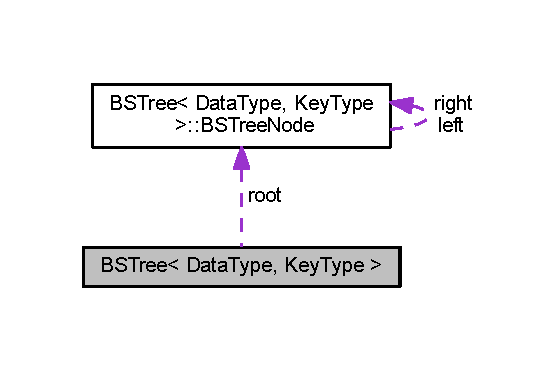
\includegraphics[width=268pt]{class_b_s_tree__coll__graph}
\end{center}
\end{figure}
\subsection*{Classes}
\begin{DoxyCompactItemize}
\item 
class \hyperlink{class_b_s_tree_1_1_b_s_tree_node}{B\+S\+Tree\+Node}
\end{DoxyCompactItemize}
\subsection*{Public Member Functions}
\begin{DoxyCompactItemize}
\item 
\hyperlink{class_b_s_tree_a4513fc6697f5e51bff8e7c448b446c9e}{B\+S\+Tree} ()
\item 
\hyperlink{class_b_s_tree_a6658391c178cb35858c9c465e1839fb0}{B\+S\+Tree} (const \hyperlink{class_b_s_tree}{B\+S\+Tree}$<$ Data\+Type, Key\+Type $>$ \&other)
\item 
\hyperlink{class_b_s_tree}{B\+S\+Tree} \& \hyperlink{class_b_s_tree_ac36b0b564aa3c411c239d730f506f448}{operator=} (const \hyperlink{class_b_s_tree}{B\+S\+Tree}$<$ Data\+Type, Key\+Type $>$ \&other)
\item 
\hyperlink{class_b_s_tree_a968c51c539f4ae41357c78b6a60fea4c}{$\sim$\+B\+S\+Tree} ()
\item 
void \hyperlink{class_b_s_tree_a3136c063de9adf6f55e524ad099df62f}{insert} (const Data\+Type \&new\+\_\+data\+\_\+item)
\item 
bool \hyperlink{class_b_s_tree_a464aa205470b150038ff35dfa01d89b8}{retrieve} (const Key\+Type \&search\+\_\+key, Data\+Type \&search\+\_\+data\+\_\+item) const
\item 
bool \hyperlink{class_b_s_tree_a7750c081fd047304b6ded5f2df65b3f3}{remove} (const Key\+Type \&delete\+\_\+key)
\item 
void \hyperlink{class_b_s_tree_a0f0b3362a2b927092a464cb37edf59b3}{write\+Keys} () const
\item 
void \hyperlink{class_b_s_tree_a926822d08f3d0321603f9fafd2254b16}{clear} ()
\item 
bool \hyperlink{class_b_s_tree_aa79c2c24f8a4068dd01526674016b861}{is\+Empty} () const
\item 
void \hyperlink{class_b_s_tree_a66690333188606d533e4ad182922d9e1}{show\+Structure} () const
\item 
int \hyperlink{class_b_s_tree_a9e8f8c02f31a9ed55458b569dd809d62}{get\+Height} () const
\item 
int \hyperlink{class_b_s_tree_a138977042d1d7cbaa363fbcf435a1e88}{get\+Count} () const
\end{DoxyCompactItemize}
\subsection*{Protected Member Functions}
\begin{DoxyCompactItemize}
\item 
bool \hyperlink{class_b_s_tree_a4bd9d8e6357091ea72da7f62e2ee9577}{remove\+\_\+helper} (\hyperlink{class_b_s_tree_1_1_b_s_tree_node}{B\+S\+Tree\+Node} $\ast$\&n, const Key\+Type \&delete\+\_\+key)
\item 
void \hyperlink{class_b_s_tree_a0c759512b61b88b824266d501beaf842}{clear\+\_\+helper} (\hyperlink{class_b_s_tree_1_1_b_s_tree_node}{B\+S\+Tree\+Node} $\ast$n)
\item 
bool \hyperlink{class_b_s_tree_ae8721d0a76719bc95e6b48420b5be302}{retrieve\+\_\+helper} (\hyperlink{class_b_s_tree_1_1_b_s_tree_node}{B\+S\+Tree\+Node} $\ast$n, const Key\+Type \&search\+\_\+key, Data\+Type \&search\+\_\+data\+\_\+item) const
\item 
int \hyperlink{class_b_s_tree_ad8a9303c63c71724cc1bba081edce42a}{get\+\_\+height\+\_\+helper} (\hyperlink{class_b_s_tree_1_1_b_s_tree_node}{B\+S\+Tree\+Node} $\ast$n) const
\item 
int \hyperlink{class_b_s_tree_a8b7d2aea1aef9e8abf213cfaaa9230ed}{get\+\_\+count\+\_\+helper} (\hyperlink{class_b_s_tree_1_1_b_s_tree_node}{B\+S\+Tree\+Node} $\ast$n) const
\item 
void \hyperlink{class_b_s_tree_a7423df4da3dd2035e681a67c321ec719}{copy\+\_\+tree} (const \hyperlink{class_b_s_tree}{B\+S\+Tree}$<$ Data\+Type, Key\+Type $>$ \&other\+\_\+tree)
\item 
void \hyperlink{class_b_s_tree_a735864f670b952c5bb2bc2550ade3a72}{show\+\_\+helper} (\hyperlink{class_b_s_tree_1_1_b_s_tree_node}{B\+S\+Tree\+Node} $\ast$n, int level) const
\item 
void \hyperlink{class_b_s_tree_a79d1cab6032e8be7484591990249c9d6}{insert\+\_\+helper} (\hyperlink{class_b_s_tree_1_1_b_s_tree_node}{B\+S\+Tree\+Node} $\ast$\&n, const Data\+Type \&new\+\_\+data\+\_\+item)
\item 
void \hyperlink{class_b_s_tree_a57b4fd45e3710cc24d63df9b80bae36d}{copy\+\_\+tree\+\_\+helper} (\hyperlink{class_b_s_tree_1_1_b_s_tree_node}{B\+S\+Tree\+Node} $\ast$\&n, const \hyperlink{class_b_s_tree_1_1_b_s_tree_node}{B\+S\+Tree\+Node} $\ast$other\+\_\+pointer)
\item 
void \hyperlink{class_b_s_tree_af3a79c41f7799cf123438f9449cf3ebb}{write\+\_\+keys\+\_\+helper} (\hyperlink{class_b_s_tree_1_1_b_s_tree_node}{B\+S\+Tree\+Node} $\ast$n) const
\end{DoxyCompactItemize}
\subsection*{Protected Attributes}
\begin{DoxyCompactItemize}
\item 
\hyperlink{class_b_s_tree_1_1_b_s_tree_node}{B\+S\+Tree\+Node} $\ast$ \hyperlink{class_b_s_tree_a83534afce9094181ac031f9f596a8625}{root}
\end{DoxyCompactItemize}


\subsection{Constructor \& Destructor Documentation}
\hypertarget{class_b_s_tree_a4513fc6697f5e51bff8e7c448b446c9e}{}\label{class_b_s_tree_a4513fc6697f5e51bff8e7c448b446c9e} 
\index{B\+S\+Tree@{B\+S\+Tree}!B\+S\+Tree@{B\+S\+Tree}}
\index{B\+S\+Tree@{B\+S\+Tree}!B\+S\+Tree@{B\+S\+Tree}}
\subsubsection{\texorpdfstring{B\+S\+Tree()}{BSTree()}\hspace{0.1cm}{\footnotesize\ttfamily [1/2]}}
{\footnotesize\ttfamily template$<$typename Data\+Type , typename Key\+Type $>$ \\
\hyperlink{class_b_s_tree}{B\+S\+Tree}$<$ Data\+Type, Key\+Type $>$\+::\hyperlink{class_b_s_tree}{B\+S\+Tree} (\begin{DoxyParamCaption}{ }\end{DoxyParamCaption})}


\begin{DoxyCode}
00042 \{
00043     \hyperlink{class_b_s_tree_a83534afce9094181ac031f9f596a8625}{root} = NULL;
00044 \}
\end{DoxyCode}
\hypertarget{class_b_s_tree_a6658391c178cb35858c9c465e1839fb0}{}\label{class_b_s_tree_a6658391c178cb35858c9c465e1839fb0} 
\index{B\+S\+Tree@{B\+S\+Tree}!B\+S\+Tree@{B\+S\+Tree}}
\index{B\+S\+Tree@{B\+S\+Tree}!B\+S\+Tree@{B\+S\+Tree}}
\subsubsection{\texorpdfstring{B\+S\+Tree()}{BSTree()}\hspace{0.1cm}{\footnotesize\ttfamily [2/2]}}
{\footnotesize\ttfamily template$<$typename Data\+Type , typename Key\+Type $>$ \\
\hyperlink{class_b_s_tree}{B\+S\+Tree}$<$ Data\+Type, Key\+Type $>$\+::\hyperlink{class_b_s_tree}{B\+S\+Tree} (\begin{DoxyParamCaption}\item[{const \hyperlink{class_b_s_tree}{B\+S\+Tree}$<$ Data\+Type, Key\+Type $>$ \&}]{other }\end{DoxyParamCaption})}


\begin{DoxyCode}
00054 \{
00055     \hyperlink{class_b_s_tree_a83534afce9094181ac031f9f596a8625}{root} = NULL;
00056     \hyperlink{class_b_s_tree_a7423df4da3dd2035e681a67c321ec719}{copy\_tree}(source);
00057 \}
\end{DoxyCode}
\hypertarget{class_b_s_tree_a968c51c539f4ae41357c78b6a60fea4c}{}\label{class_b_s_tree_a968c51c539f4ae41357c78b6a60fea4c} 
\index{B\+S\+Tree@{B\+S\+Tree}!````~B\+S\+Tree@{$\sim$\+B\+S\+Tree}}
\index{````~B\+S\+Tree@{$\sim$\+B\+S\+Tree}!B\+S\+Tree@{B\+S\+Tree}}
\subsubsection{\texorpdfstring{$\sim$\+B\+S\+Tree()}{~BSTree()}}
{\footnotesize\ttfamily template$<$typename Data\+Type , typename Key\+Type $>$ \\
\hyperlink{class_b_s_tree}{B\+S\+Tree}$<$ Data\+Type, Key\+Type $>$\+::$\sim$\hyperlink{class_b_s_tree}{B\+S\+Tree} (\begin{DoxyParamCaption}{ }\end{DoxyParamCaption})}


\begin{DoxyCode}
00116 \{
00117     \hyperlink{class_b_s_tree_a926822d08f3d0321603f9fafd2254b16}{clear}();
00118 \}
\end{DoxyCode}


\subsection{Member Function Documentation}
\hypertarget{class_b_s_tree_a926822d08f3d0321603f9fafd2254b16}{}\label{class_b_s_tree_a926822d08f3d0321603f9fafd2254b16} 
\index{B\+S\+Tree@{B\+S\+Tree}!clear@{clear}}
\index{clear@{clear}!B\+S\+Tree@{B\+S\+Tree}}
\subsubsection{\texorpdfstring{clear()}{clear()}}
{\footnotesize\ttfamily template$<$typename Data\+Type , typename Key\+Type $>$ \\
void \hyperlink{class_b_s_tree}{B\+S\+Tree}$<$ Data\+Type, Key\+Type $>$\+::clear (\begin{DoxyParamCaption}{ }\end{DoxyParamCaption})}


\begin{DoxyCode}
00299 \{
00300     \hyperlink{class_b_s_tree_a0c759512b61b88b824266d501beaf842}{clear\_helper}(\hyperlink{class_b_s_tree_a83534afce9094181ac031f9f596a8625}{root});
00301     \hyperlink{class_b_s_tree_a83534afce9094181ac031f9f596a8625}{root} = 0;
00302 \}
\end{DoxyCode}
\hypertarget{class_b_s_tree_a0c759512b61b88b824266d501beaf842}{}\label{class_b_s_tree_a0c759512b61b88b824266d501beaf842} 
\index{B\+S\+Tree@{B\+S\+Tree}!clear\+\_\+helper@{clear\+\_\+helper}}
\index{clear\+\_\+helper@{clear\+\_\+helper}!B\+S\+Tree@{B\+S\+Tree}}
\subsubsection{\texorpdfstring{clear\+\_\+helper()}{clear\_helper()}}
{\footnotesize\ttfamily template$<$typename Data\+Type , typename Key\+Type $>$ \\
void \hyperlink{class_b_s_tree}{B\+S\+Tree}$<$ Data\+Type, Key\+Type $>$\+::clear\+\_\+helper (\begin{DoxyParamCaption}\item[{\hyperlink{class_b_s_tree_1_1_b_s_tree_node}{B\+S\+Tree\+Node} $\ast$}]{n }\end{DoxyParamCaption})\hspace{0.3cm}{\ttfamily [protected]}}


\begin{DoxyCode}
00312 \{
00313     \textcolor{keywordflow}{if} (n != 0)
00314     \{
00315         \hyperlink{class_b_s_tree_a0c759512b61b88b824266d501beaf842}{clear\_helper}(n->left);
00316         \hyperlink{class_b_s_tree_a0c759512b61b88b824266d501beaf842}{clear\_helper}(n->right);
00317         \textcolor{keyword}{delete} n;
00318     \}
00319 \}
\end{DoxyCode}
\hypertarget{class_b_s_tree_a7423df4da3dd2035e681a67c321ec719}{}\label{class_b_s_tree_a7423df4da3dd2035e681a67c321ec719} 
\index{B\+S\+Tree@{B\+S\+Tree}!copy\+\_\+tree@{copy\+\_\+tree}}
\index{copy\+\_\+tree@{copy\+\_\+tree}!B\+S\+Tree@{B\+S\+Tree}}
\subsubsection{\texorpdfstring{copy\+\_\+tree()}{copy\_tree()}}
{\footnotesize\ttfamily template$<$typename Data\+Type , typename Key\+Type $>$ \\
void \hyperlink{class_b_s_tree}{B\+S\+Tree}$<$ Data\+Type, Key\+Type $>$\+::copy\+\_\+tree (\begin{DoxyParamCaption}\item[{const \hyperlink{class_b_s_tree}{B\+S\+Tree}$<$ Data\+Type, Key\+Type $>$ \&}]{other\+\_\+tree }\end{DoxyParamCaption})\hspace{0.3cm}{\ttfamily [protected]}}


\begin{DoxyCode}
00088 \{
00089     \hyperlink{class_b_s_tree_a57b4fd45e3710cc24d63df9b80bae36d}{copy\_tree\_helper}(\hyperlink{class_b_s_tree_a83534afce9094181ac031f9f596a8625}{root}, source\_tree.root);
00090 \}
\end{DoxyCode}
\hypertarget{class_b_s_tree_a57b4fd45e3710cc24d63df9b80bae36d}{}\label{class_b_s_tree_a57b4fd45e3710cc24d63df9b80bae36d} 
\index{B\+S\+Tree@{B\+S\+Tree}!copy\+\_\+tree\+\_\+helper@{copy\+\_\+tree\+\_\+helper}}
\index{copy\+\_\+tree\+\_\+helper@{copy\+\_\+tree\+\_\+helper}!B\+S\+Tree@{B\+S\+Tree}}
\subsubsection{\texorpdfstring{copy\+\_\+tree\+\_\+helper()}{copy\_tree\_helper()}}
{\footnotesize\ttfamily template$<$typename Data\+Type , typename Key\+Type $>$ \\
void \hyperlink{class_b_s_tree}{B\+S\+Tree}$<$ Data\+Type, Key\+Type $>$\+::copy\+\_\+tree\+\_\+helper (\begin{DoxyParamCaption}\item[{\hyperlink{class_b_s_tree_1_1_b_s_tree_node}{B\+S\+Tree\+Node} $\ast$\&}]{n,  }\item[{const \hyperlink{class_b_s_tree_1_1_b_s_tree_node}{B\+S\+Tree\+Node} $\ast$}]{other\+\_\+pointer }\end{DoxyParamCaption})\hspace{0.3cm}{\ttfamily [protected]}}


\begin{DoxyCode}
00100 \{
00101     \textcolor{keywordflow}{if} (n != 0) \{
00102         n = \textcolor{keyword}{new} BSTreeNode(source\_pointer->dataItem, 0, 0);
00103         \hyperlink{class_b_s_tree_a57b4fd45e3710cc24d63df9b80bae36d}{copy\_tree\_helper}(n->left, source\_pointer->left);
00104         \hyperlink{class_b_s_tree_a57b4fd45e3710cc24d63df9b80bae36d}{copy\_tree\_helper}(n->right, source\_pointer->right);
00105     \}
00106 \}
\end{DoxyCode}
\hypertarget{class_b_s_tree_a8b7d2aea1aef9e8abf213cfaaa9230ed}{}\label{class_b_s_tree_a8b7d2aea1aef9e8abf213cfaaa9230ed} 
\index{B\+S\+Tree@{B\+S\+Tree}!get\+\_\+count\+\_\+helper@{get\+\_\+count\+\_\+helper}}
\index{get\+\_\+count\+\_\+helper@{get\+\_\+count\+\_\+helper}!B\+S\+Tree@{B\+S\+Tree}}
\subsubsection{\texorpdfstring{get\+\_\+count\+\_\+helper()}{get\_count\_helper()}}
{\footnotesize\ttfamily template$<$typename Data\+Type , typename Key\+Type $>$ \\
int \hyperlink{class_b_s_tree}{B\+S\+Tree}$<$ Data\+Type, Key\+Type $>$\+::get\+\_\+count\+\_\+helper (\begin{DoxyParamCaption}\item[{\hyperlink{class_b_s_tree_1_1_b_s_tree_node}{B\+S\+Tree\+Node} $\ast$}]{n }\end{DoxyParamCaption}) const\hspace{0.3cm}{\ttfamily [protected]}}


\begin{DoxyCode}
00436 \{
00437     \textcolor{keywordflow}{if} (n == 0) 
00438     \{
00439         \textcolor{keywordflow}{return} 0;
00440     \}
00441 
00442     \textcolor{keywordflow}{return} \hyperlink{class_b_s_tree_a8b7d2aea1aef9e8abf213cfaaa9230ed}{get\_count\_helper}(n->left) + \hyperlink{class_b_s_tree_a8b7d2aea1aef9e8abf213cfaaa9230ed}{get\_count\_helper}(n->right) + 1;
00443 \}
\end{DoxyCode}
\hypertarget{class_b_s_tree_ad8a9303c63c71724cc1bba081edce42a}{}\label{class_b_s_tree_ad8a9303c63c71724cc1bba081edce42a} 
\index{B\+S\+Tree@{B\+S\+Tree}!get\+\_\+height\+\_\+helper@{get\+\_\+height\+\_\+helper}}
\index{get\+\_\+height\+\_\+helper@{get\+\_\+height\+\_\+helper}!B\+S\+Tree@{B\+S\+Tree}}
\subsubsection{\texorpdfstring{get\+\_\+height\+\_\+helper()}{get\_height\_helper()}}
{\footnotesize\ttfamily template$<$typename Data\+Type , typename Key\+Type $>$ \\
int \hyperlink{class_b_s_tree}{B\+S\+Tree}$<$ Data\+Type, Key\+Type $>$\+::get\+\_\+height\+\_\+helper (\begin{DoxyParamCaption}\item[{\hyperlink{class_b_s_tree_1_1_b_s_tree_node}{B\+S\+Tree\+Node} $\ast$}]{n }\end{DoxyParamCaption}) const\hspace{0.3cm}{\ttfamily [protected]}}


\begin{DoxyCode}
00399 \{
00400     \textcolor{keywordtype}{int} length\_of\_left, length\_of\_right, result;   
00401 
00402     \textcolor{keywordflow}{if} (n == 0)
00403         result = 0;                    
00404     \textcolor{keywordflow}{else}
00405     \{
00406         length\_of\_left = \hyperlink{class_b_s_tree_ad8a9303c63c71724cc1bba081edce42a}{get\_height\_helper}(n->left) + 1;    
00407         length\_of\_right = \hyperlink{class_b_s_tree_ad8a9303c63c71724cc1bba081edce42a}{get\_height\_helper}(n->right) + 1;   
00408         \textcolor{keywordflow}{if} (length\_of\_left >= length\_of\_right)                  
00409             result = length\_of\_left;
00410         \textcolor{keywordflow}{else}
00411             result = length\_of\_right;
00412     \}
00413 
00414     \textcolor{keywordflow}{return} result;
00415 \}
\end{DoxyCode}
\hypertarget{class_b_s_tree_a138977042d1d7cbaa363fbcf435a1e88}{}\label{class_b_s_tree_a138977042d1d7cbaa363fbcf435a1e88} 
\index{B\+S\+Tree@{B\+S\+Tree}!get\+Count@{get\+Count}}
\index{get\+Count@{get\+Count}!B\+S\+Tree@{B\+S\+Tree}}
\subsubsection{\texorpdfstring{get\+Count()}{getCount()}}
{\footnotesize\ttfamily template$<$typename Data\+Type , typename Key\+Type $>$ \\
int \hyperlink{class_b_s_tree}{B\+S\+Tree}$<$ Data\+Type, Key\+Type $>$\+::get\+Count (\begin{DoxyParamCaption}{ }\end{DoxyParamCaption}) const}


\begin{DoxyCode}
00424 \{
00425     \textcolor{keywordflow}{return} \hyperlink{class_b_s_tree_a8b7d2aea1aef9e8abf213cfaaa9230ed}{get\_count\_helper}(\hyperlink{class_b_s_tree_a83534afce9094181ac031f9f596a8625}{root});
00426 \}
\end{DoxyCode}
\hypertarget{class_b_s_tree_a9e8f8c02f31a9ed55458b569dd809d62}{}\label{class_b_s_tree_a9e8f8c02f31a9ed55458b569dd809d62} 
\index{B\+S\+Tree@{B\+S\+Tree}!get\+Height@{get\+Height}}
\index{get\+Height@{get\+Height}!B\+S\+Tree@{B\+S\+Tree}}
\subsubsection{\texorpdfstring{get\+Height()}{getHeight()}}
{\footnotesize\ttfamily template$<$typename Data\+Type , typename Key\+Type $>$ \\
int \hyperlink{class_b_s_tree}{B\+S\+Tree}$<$ Data\+Type, Key\+Type $>$\+::get\+Height (\begin{DoxyParamCaption}{ }\end{DoxyParamCaption}) const}


\begin{DoxyCode}
00387 \{
00388     \textcolor{keywordflow}{return} \hyperlink{class_b_s_tree_ad8a9303c63c71724cc1bba081edce42a}{get\_height\_helper}(\hyperlink{class_b_s_tree_a83534afce9094181ac031f9f596a8625}{root});
00389 \}
\end{DoxyCode}
\hypertarget{class_b_s_tree_a3136c063de9adf6f55e524ad099df62f}{}\label{class_b_s_tree_a3136c063de9adf6f55e524ad099df62f} 
\index{B\+S\+Tree@{B\+S\+Tree}!insert@{insert}}
\index{insert@{insert}!B\+S\+Tree@{B\+S\+Tree}}
\subsubsection{\texorpdfstring{insert()}{insert()}}
{\footnotesize\ttfamily template$<$typename Data\+Type , typename Key\+Type $>$ \\
void \hyperlink{class_b_s_tree}{B\+S\+Tree}$<$ Data\+Type, Key\+Type $>$\+::insert (\begin{DoxyParamCaption}\item[{const Data\+Type \&}]{new\+\_\+data\+\_\+item }\end{DoxyParamCaption})}


\begin{DoxyCode}
00128 \{
00129     \hyperlink{class_b_s_tree_a79d1cab6032e8be7484591990249c9d6}{insert\_helper}(\hyperlink{class_b_s_tree_a83534afce9094181ac031f9f596a8625}{root}, new\_data\_item);
00130 \}
\end{DoxyCode}
Here is the caller graph for this function\+:
\nopagebreak
\begin{figure}[H]
\begin{center}
\leavevmode
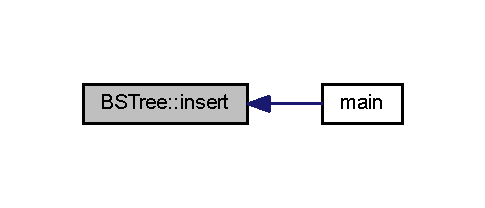
\includegraphics[width=233pt]{class_b_s_tree_a3136c063de9adf6f55e524ad099df62f_icgraph}
\end{center}
\end{figure}
\hypertarget{class_b_s_tree_a79d1cab6032e8be7484591990249c9d6}{}\label{class_b_s_tree_a79d1cab6032e8be7484591990249c9d6} 
\index{B\+S\+Tree@{B\+S\+Tree}!insert\+\_\+helper@{insert\+\_\+helper}}
\index{insert\+\_\+helper@{insert\+\_\+helper}!B\+S\+Tree@{B\+S\+Tree}}
\subsubsection{\texorpdfstring{insert\+\_\+helper()}{insert\_helper()}}
{\footnotesize\ttfamily template$<$typename Data\+Type , typename Key\+Type $>$ \\
void \hyperlink{class_b_s_tree}{B\+S\+Tree}$<$ Data\+Type, Key\+Type $>$\+::insert\+\_\+helper (\begin{DoxyParamCaption}\item[{\hyperlink{class_b_s_tree_1_1_b_s_tree_node}{B\+S\+Tree\+Node} $\ast$\&}]{n,  }\item[{const Data\+Type \&}]{new\+\_\+data\+\_\+item }\end{DoxyParamCaption})\hspace{0.3cm}{\ttfamily [protected]}}


\begin{DoxyCode}
00141 \{
00142     \textcolor{keywordflow}{if} (n == 0) \textcolor{comment}{// Insert}
00143         n = \textcolor{keyword}{new} BSTreeNode(new\_data\_item, 0, 0);
00144     \textcolor{keywordflow}{else} \textcolor{keywordflow}{if} (new\_data\_item.getKey() < n->dataItem.getKey())
00145         \hyperlink{class_b_s_tree_a79d1cab6032e8be7484591990249c9d6}{insert\_helper}(n->left, new\_data\_item);
00146     \textcolor{keywordflow}{else} \textcolor{keywordflow}{if} (new\_data\_item.getKey() > n->dataItem.getKey())
00147         \hyperlink{class_b_s_tree_a79d1cab6032e8be7484591990249c9d6}{insert\_helper}(n->right, new\_data\_item);
00148     \textcolor{keywordflow}{else}
00149         n->dataItem = new\_data\_item;
00150 \}
\end{DoxyCode}
\hypertarget{class_b_s_tree_aa79c2c24f8a4068dd01526674016b861}{}\label{class_b_s_tree_aa79c2c24f8a4068dd01526674016b861} 
\index{B\+S\+Tree@{B\+S\+Tree}!is\+Empty@{is\+Empty}}
\index{is\+Empty@{is\+Empty}!B\+S\+Tree@{B\+S\+Tree}}
\subsubsection{\texorpdfstring{is\+Empty()}{isEmpty()}}
{\footnotesize\ttfamily template$<$typename Data\+Type , typename Key\+Type $>$ \\
bool \hyperlink{class_b_s_tree}{B\+S\+Tree}$<$ Data\+Type, Key\+Type $>$\+::is\+Empty (\begin{DoxyParamCaption}{ }\end{DoxyParamCaption}) const}


\begin{DoxyCode}
00329 \{
00330     \textcolor{keywordflow}{return} \hyperlink{class_b_s_tree_a83534afce9094181ac031f9f596a8625}{root} == 0;
00331 \}
\end{DoxyCode}
\hypertarget{class_b_s_tree_ac36b0b564aa3c411c239d730f506f448}{}\label{class_b_s_tree_ac36b0b564aa3c411c239d730f506f448} 
\index{B\+S\+Tree@{B\+S\+Tree}!operator=@{operator=}}
\index{operator=@{operator=}!B\+S\+Tree@{B\+S\+Tree}}
\subsubsection{\texorpdfstring{operator=()}{operator=()}}
{\footnotesize\ttfamily template$<$typename Data\+Type , typename Key\+Type $>$ \\
\hyperlink{class_b_s_tree}{B\+S\+Tree}$<$ Data\+Type, Key\+Type $>$ \& \hyperlink{class_b_s_tree}{B\+S\+Tree}$<$ Data\+Type, Key\+Type $>$\+::operator= (\begin{DoxyParamCaption}\item[{const \hyperlink{class_b_s_tree}{B\+S\+Tree}$<$ Data\+Type, Key\+Type $>$ \&}]{other }\end{DoxyParamCaption})}


\begin{DoxyCode}
00067 \{
00068     \textcolor{keywordflow}{if} (\textcolor{keyword}{this} != &source\_tree)
00069     \{
00070         \hyperlink{class_b_s_tree_a926822d08f3d0321603f9fafd2254b16}{clear}();
00071         \hyperlink{class_b_s_tree_a7423df4da3dd2035e681a67c321ec719}{copy\_tree}(source\_tree);
00072         \textcolor{keywordflow}{return} *\textcolor{keyword}{this};
00073     \}
00074     \textcolor{keywordflow}{else}
00075     \{
00076         \textcolor{keywordflow}{return} *\textcolor{keyword}{this};
00077     \}
00078 \}
\end{DoxyCode}
\hypertarget{class_b_s_tree_a7750c081fd047304b6ded5f2df65b3f3}{}\label{class_b_s_tree_a7750c081fd047304b6ded5f2df65b3f3} 
\index{B\+S\+Tree@{B\+S\+Tree}!remove@{remove}}
\index{remove@{remove}!B\+S\+Tree@{B\+S\+Tree}}
\subsubsection{\texorpdfstring{remove()}{remove()}}
{\footnotesize\ttfamily template$<$typename Data\+Type , typename Key\+Type $>$ \\
bool \hyperlink{class_b_s_tree}{B\+S\+Tree}$<$ Data\+Type, Key\+Type $>$\+::remove (\begin{DoxyParamCaption}\item[{const Key\+Type \&}]{delete\+\_\+key }\end{DoxyParamCaption})}


\begin{DoxyCode}
00207 \{
00208     \textcolor{keywordflow}{return} \hyperlink{class_b_s_tree_a4bd9d8e6357091ea72da7f62e2ee9577}{remove\_helper}(\hyperlink{class_b_s_tree_a83534afce9094181ac031f9f596a8625}{root}, delete\_key);
00209 \}
\end{DoxyCode}
\hypertarget{class_b_s_tree_a4bd9d8e6357091ea72da7f62e2ee9577}{}\label{class_b_s_tree_a4bd9d8e6357091ea72da7f62e2ee9577} 
\index{B\+S\+Tree@{B\+S\+Tree}!remove\+\_\+helper@{remove\+\_\+helper}}
\index{remove\+\_\+helper@{remove\+\_\+helper}!B\+S\+Tree@{B\+S\+Tree}}
\subsubsection{\texorpdfstring{remove\+\_\+helper()}{remove\_helper()}}
{\footnotesize\ttfamily template$<$typename Data\+Type , typename Key\+Type $>$ \\
bool \hyperlink{class_b_s_tree}{B\+S\+Tree}$<$ Data\+Type, Key\+Type $>$\+::remove\+\_\+helper (\begin{DoxyParamCaption}\item[{\hyperlink{class_b_s_tree_1_1_b_s_tree_node}{B\+S\+Tree\+Node} $\ast$\&}]{n,  }\item[{const Key\+Type \&}]{delete\+\_\+key }\end{DoxyParamCaption})\hspace{0.3cm}{\ttfamily [protected]}}


\begin{DoxyCode}
00220 \{
00221     BSTreeNode* delete\_pointer; 
00222     \textcolor{keywordtype}{int} result;                 
00223 
00224     \textcolor{keywordflow}{if} (n == 0)
00225         result = \textcolor{keyword}{false};                           
00226     \textcolor{keywordflow}{else} \textcolor{keywordflow}{if} (delete\_key < n->dataItem.getKey())
00227         result = \hyperlink{class_b_s_tree_a4bd9d8e6357091ea72da7f62e2ee9577}{remove\_helper}(n->left, delete\_key);
00228     \textcolor{keywordflow}{else} \textcolor{keywordflow}{if} (delete\_key > n->dataItem.getKey())
00229         result = \hyperlink{class_b_s_tree_a4bd9d8e6357091ea72da7f62e2ee9577}{remove\_helper}(n->right, delete\_key);
00230     \textcolor{keywordflow}{else}
00231     \{                                            
00232         delete\_pointer = n;
00233         \textcolor{keywordflow}{if} (n->left == 0)
00234         \{
00235             n = n->right;                    
00236             \textcolor{keyword}{delete} delete\_pointer;
00237         \}
00238         \textcolor{keywordflow}{else} \textcolor{keywordflow}{if} (n->right == 0)
00239         \{
00240             n = n->left;                     
00241             \textcolor{keyword}{delete} delete\_pointer;
00242         \}
00243         \textcolor{keywordflow}{else}
00244             
00245         \{
00246             BSTreeNode* temp = n->left;
00247             \textcolor{keywordflow}{while} (temp->right) 
00248             \{
00249                 temp = temp->right;
00250             \}
00251             n->dataItem = temp->dataItem;
00252             \hyperlink{class_b_s_tree_a4bd9d8e6357091ea72da7f62e2ee9577}{remove\_helper}(n->left, temp->dataItem.getKey());
00253 
00254         \}
00255         result = \textcolor{keyword}{true};
00256     \}
00257 
00258     \textcolor{keywordflow}{return} result;
00259 \}
\end{DoxyCode}
\hypertarget{class_b_s_tree_a464aa205470b150038ff35dfa01d89b8}{}\label{class_b_s_tree_a464aa205470b150038ff35dfa01d89b8} 
\index{B\+S\+Tree@{B\+S\+Tree}!retrieve@{retrieve}}
\index{retrieve@{retrieve}!B\+S\+Tree@{B\+S\+Tree}}
\subsubsection{\texorpdfstring{retrieve()}{retrieve()}}
{\footnotesize\ttfamily template$<$typename Data\+Type , typename Key\+Type $>$ \\
bool \hyperlink{class_b_s_tree}{B\+S\+Tree}$<$ Data\+Type, Key\+Type $>$\+::retrieve (\begin{DoxyParamCaption}\item[{const Key\+Type \&}]{search\+\_\+key,  }\item[{Data\+Type \&}]{search\+\_\+data\+\_\+item }\end{DoxyParamCaption}) const}


\begin{DoxyCode}
00161 \{
00162     \textcolor{keywordflow}{return} \hyperlink{class_b_s_tree_ae8721d0a76719bc95e6b48420b5be302}{retrieve\_helper}(\hyperlink{class_b_s_tree_a83534afce9094181ac031f9f596a8625}{root}, search\_key, search\_data\_item);
00163 \}
\end{DoxyCode}
Here is the caller graph for this function\+:
\nopagebreak
\begin{figure}[H]
\begin{center}
\leavevmode
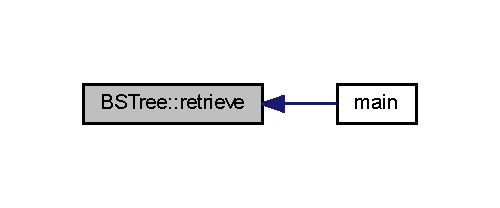
\includegraphics[width=240pt]{class_b_s_tree_a464aa205470b150038ff35dfa01d89b8_icgraph}
\end{center}
\end{figure}
\hypertarget{class_b_s_tree_ae8721d0a76719bc95e6b48420b5be302}{}\label{class_b_s_tree_ae8721d0a76719bc95e6b48420b5be302} 
\index{B\+S\+Tree@{B\+S\+Tree}!retrieve\+\_\+helper@{retrieve\+\_\+helper}}
\index{retrieve\+\_\+helper@{retrieve\+\_\+helper}!B\+S\+Tree@{B\+S\+Tree}}
\subsubsection{\texorpdfstring{retrieve\+\_\+helper()}{retrieve\_helper()}}
{\footnotesize\ttfamily template$<$typename Data\+Type , typename Key\+Type $>$ \\
bool \hyperlink{class_b_s_tree}{B\+S\+Tree}$<$ Data\+Type, Key\+Type $>$\+::retrieve\+\_\+helper (\begin{DoxyParamCaption}\item[{\hyperlink{class_b_s_tree_1_1_b_s_tree_node}{B\+S\+Tree\+Node} $\ast$}]{n,  }\item[{const Key\+Type \&}]{search\+\_\+key,  }\item[{Data\+Type \&}]{search\+\_\+data\+\_\+item }\end{DoxyParamCaption}) const\hspace{0.3cm}{\ttfamily [protected]}}


\begin{DoxyCode}
00175 \{
00176     \textcolor{keywordtype}{bool} result;
00177 
00178     \textcolor{keywordflow}{if} (n == 0)
00179     \{
00180         result = \textcolor{keyword}{false};
00181     \}
00182     \textcolor{keywordflow}{else} \textcolor{keywordflow}{if} (search\_key < n->dataItem.getKey())
00183     \{
00184         result = \hyperlink{class_b_s_tree_ae8721d0a76719bc95e6b48420b5be302}{retrieve\_helper}(n->left, search\_key, search\_data\_item);
00185     \}
00186     \textcolor{keywordflow}{else} \textcolor{keywordflow}{if} (search\_key > n->dataItem.getKey())
00187     \{
00188         result = \hyperlink{class_b_s_tree_ae8721d0a76719bc95e6b48420b5be302}{retrieve\_helper}(n->right, search\_key, search\_data\_item);
00189     \}
00190     \textcolor{keywordflow}{else}
00191     \{
00192         search\_data\_item = n->dataItem;
00193         result = \textcolor{keyword}{true};
00194     \}
00195 
00196     \textcolor{keywordflow}{return} result;
00197 \}
\end{DoxyCode}
\hypertarget{class_b_s_tree_a735864f670b952c5bb2bc2550ade3a72}{}\label{class_b_s_tree_a735864f670b952c5bb2bc2550ade3a72} 
\index{B\+S\+Tree@{B\+S\+Tree}!show\+\_\+helper@{show\+\_\+helper}}
\index{show\+\_\+helper@{show\+\_\+helper}!B\+S\+Tree@{B\+S\+Tree}}
\subsubsection{\texorpdfstring{show\+\_\+helper()}{show\_helper()}}
{\footnotesize\ttfamily template$<$typename Data\+Type , typename Key\+Type $>$ \\
void \hyperlink{class_b_s_tree}{B\+S\+Tree}$<$ Data\+Type, Key\+Type $>$\+::show\+\_\+helper (\begin{DoxyParamCaption}\item[{\hyperlink{class_b_s_tree_1_1_b_s_tree_node}{B\+S\+Tree\+Node} $\ast$}]{n,  }\item[{int}]{level }\end{DoxyParamCaption}) const\hspace{0.3cm}{\ttfamily [protected]}}


\begin{DoxyCode}
00360 \{
00361     \textcolor{keywordflow}{if} (n != 0)
00362     \{
00363         \hyperlink{class_b_s_tree_a735864f670b952c5bb2bc2550ade3a72}{show\_helper}(n->right, level + 1);         
00364         \textcolor{keywordflow}{for} (\textcolor{keywordtype}{int} i = 0; i < level; i++)    
00365             cout << \textcolor{stringliteral}{"\(\backslash\)t"};
00366         cout << \textcolor{stringliteral}{" "} << n->dataItem.getKey();   
00367         \textcolor{keywordflow}{if} ((n->left != 0) &&          
00368             (n->right != 0))
00369             cout << \textcolor{stringliteral}{"<"};
00370         \textcolor{keywordflow}{else} \textcolor{keywordflow}{if} (n->right != 0)
00371             cout << \textcolor{stringliteral}{"/"};
00372         \textcolor{keywordflow}{else} \textcolor{keywordflow}{if} (n->left != 0)
00373             cout << \textcolor{stringliteral}{"\(\backslash\)\(\backslash\)"};
00374         cout << endl;
00375         \hyperlink{class_b_s_tree_a735864f670b952c5bb2bc2550ade3a72}{show\_helper}(n->left, level + 1);          
00376     \}
00377 \}
\end{DoxyCode}
\hypertarget{class_b_s_tree_a66690333188606d533e4ad182922d9e1}{}\label{class_b_s_tree_a66690333188606d533e4ad182922d9e1} 
\index{B\+S\+Tree@{B\+S\+Tree}!show\+Structure@{show\+Structure}}
\index{show\+Structure@{show\+Structure}!B\+S\+Tree@{B\+S\+Tree}}
\subsubsection{\texorpdfstring{show\+Structure()}{showStructure()}}
{\footnotesize\ttfamily template$<$typename Data\+Type , typename Key\+Type $>$ \\
void \hyperlink{class_b_s_tree}{B\+S\+Tree}$<$ Data\+Type, Key\+Type $>$\+::show\+Structure (\begin{DoxyParamCaption}{ }\end{DoxyParamCaption}) const}


\begin{DoxyCode}
00341 \{
00342     \textcolor{keywordflow}{if} (\hyperlink{class_b_s_tree_a83534afce9094181ac031f9f596a8625}{root} == 0)
00343         cout << \textcolor{stringliteral}{"Tree is empty."} << endl;
00344     \textcolor{keywordflow}{else}
00345     \{
00346         cout << endl;
00347         \hyperlink{class_b_s_tree_a735864f670b952c5bb2bc2550ade3a72}{show\_helper}(\hyperlink{class_b_s_tree_a83534afce9094181ac031f9f596a8625}{root}, 1);
00348         cout << endl;
00349     \}
00350 \}
\end{DoxyCode}
\hypertarget{class_b_s_tree_af3a79c41f7799cf123438f9449cf3ebb}{}\label{class_b_s_tree_af3a79c41f7799cf123438f9449cf3ebb} 
\index{B\+S\+Tree@{B\+S\+Tree}!write\+\_\+keys\+\_\+helper@{write\+\_\+keys\+\_\+helper}}
\index{write\+\_\+keys\+\_\+helper@{write\+\_\+keys\+\_\+helper}!B\+S\+Tree@{B\+S\+Tree}}
\subsubsection{\texorpdfstring{write\+\_\+keys\+\_\+helper()}{write\_keys\_helper()}}
{\footnotesize\ttfamily template$<$typename Data\+Type , typename Key\+Type $>$ \\
void \hyperlink{class_b_s_tree}{B\+S\+Tree}$<$ Data\+Type, Key\+Type $>$\+::write\+\_\+keys\+\_\+helper (\begin{DoxyParamCaption}\item[{\hyperlink{class_b_s_tree_1_1_b_s_tree_node}{B\+S\+Tree\+Node} $\ast$}]{n }\end{DoxyParamCaption}) const\hspace{0.3cm}{\ttfamily [protected]}}


\begin{DoxyCode}
00282 \{
00283     \textcolor{keywordflow}{if} (n != 0)
00284     \{
00285         \hyperlink{class_b_s_tree_af3a79c41f7799cf123438f9449cf3ebb}{write\_keys\_helper}(n->left);
00286         cout << n->dataItem.getKey() << \textcolor{stringliteral}{" "};
00287         \hyperlink{class_b_s_tree_af3a79c41f7799cf123438f9449cf3ebb}{write\_keys\_helper}(n->right);
00288     \}
00289 \}
\end{DoxyCode}
\hypertarget{class_b_s_tree_a0f0b3362a2b927092a464cb37edf59b3}{}\label{class_b_s_tree_a0f0b3362a2b927092a464cb37edf59b3} 
\index{B\+S\+Tree@{B\+S\+Tree}!write\+Keys@{write\+Keys}}
\index{write\+Keys@{write\+Keys}!B\+S\+Tree@{B\+S\+Tree}}
\subsubsection{\texorpdfstring{write\+Keys()}{writeKeys()}}
{\footnotesize\ttfamily template$<$typename Data\+Type , typename Key\+Type $>$ \\
void \hyperlink{class_b_s_tree}{B\+S\+Tree}$<$ Data\+Type, Key\+Type $>$\+::write\+Keys (\begin{DoxyParamCaption}{ }\end{DoxyParamCaption}) const}


\begin{DoxyCode}
00269 \{
00270     \hyperlink{class_b_s_tree_af3a79c41f7799cf123438f9449cf3ebb}{write\_keys\_helper}(\hyperlink{class_b_s_tree_a83534afce9094181ac031f9f596a8625}{root});
00271     cout << endl;
00272 \}
\end{DoxyCode}
Here is the caller graph for this function\+:
\nopagebreak
\begin{figure}[H]
\begin{center}
\leavevmode
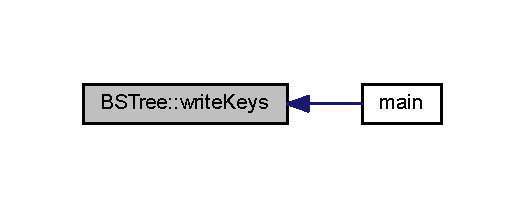
\includegraphics[width=252pt]{class_b_s_tree_a0f0b3362a2b927092a464cb37edf59b3_icgraph}
\end{center}
\end{figure}


\subsection{Member Data Documentation}
\hypertarget{class_b_s_tree_a83534afce9094181ac031f9f596a8625}{}\label{class_b_s_tree_a83534afce9094181ac031f9f596a8625} 
\index{B\+S\+Tree@{B\+S\+Tree}!root@{root}}
\index{root@{root}!B\+S\+Tree@{B\+S\+Tree}}
\subsubsection{\texorpdfstring{root}{root}}
{\footnotesize\ttfamily template$<$typename Data\+Type, class Key\+Type$>$ \\
\hyperlink{class_b_s_tree_1_1_b_s_tree_node}{B\+S\+Tree\+Node}$\ast$ \hyperlink{class_b_s_tree}{B\+S\+Tree}$<$ Data\+Type, Key\+Type $>$\+::root\hspace{0.3cm}{\ttfamily [protected]}}



The documentation for this class was generated from the following files\+:\begin{DoxyCompactItemize}
\item 
\hyperlink{_b_s_tree_8h}{B\+S\+Tree.\+h}\item 
\hyperlink{_b_s_tree_8cpp}{B\+S\+Tree.\+cpp}\end{DoxyCompactItemize}

\hypertarget{class_b_s_tree_1_1_b_s_tree_node}{}\section{B\+S\+Tree$<$ Data\+Type, Key\+Type $>$\+:\+:B\+S\+Tree\+Node Class Reference}
\label{class_b_s_tree_1_1_b_s_tree_node}\index{B\+S\+Tree$<$ Data\+Type, Key\+Type $>$\+::\+B\+S\+Tree\+Node@{B\+S\+Tree$<$ Data\+Type, Key\+Type $>$\+::\+B\+S\+Tree\+Node}}


{\ttfamily \#include $<$B\+S\+Tree.\+h$>$}



Collaboration diagram for B\+S\+Tree$<$ Data\+Type, Key\+Type $>$\+:\+:B\+S\+Tree\+Node\+:
\nopagebreak
\begin{figure}[H]
\begin{center}
\leavevmode
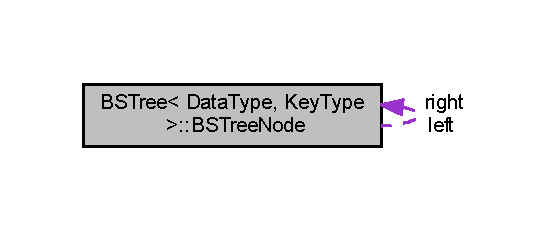
\includegraphics[width=263pt]{class_b_s_tree_1_1_b_s_tree_node__coll__graph}
\end{center}
\end{figure}
\subsection*{Public Member Functions}
\begin{DoxyCompactItemize}
\item 
\hyperlink{class_b_s_tree_1_1_b_s_tree_node_a083eecbe3e2421ca811a05e1e8ba1203}{B\+S\+Tree\+Node} (const Data\+Type \&node\+\_\+data\+\_\+item, \hyperlink{class_b_s_tree_1_1_b_s_tree_node}{B\+S\+Tree\+Node} $\ast$left\+\_\+pointer, \hyperlink{class_b_s_tree_1_1_b_s_tree_node}{B\+S\+Tree\+Node} $\ast$right\+\_\+pointer)
\end{DoxyCompactItemize}
\subsection*{Public Attributes}
\begin{DoxyCompactItemize}
\item 
Data\+Type \hyperlink{class_b_s_tree_1_1_b_s_tree_node_a507c8d6dde1b8d35d9af6b4e78f38962}{data\+Item}
\item 
\hyperlink{class_b_s_tree_1_1_b_s_tree_node}{B\+S\+Tree\+Node} $\ast$ \hyperlink{class_b_s_tree_1_1_b_s_tree_node_a7a90150dd249432e240dc363955c5ca1}{left}
\item 
\hyperlink{class_b_s_tree_1_1_b_s_tree_node}{B\+S\+Tree\+Node} $\ast$ \hyperlink{class_b_s_tree_1_1_b_s_tree_node_a8d7bfd0208a562c8b8ab332e1d796563}{right}
\end{DoxyCompactItemize}


\subsection{Constructor \& Destructor Documentation}
\hypertarget{class_b_s_tree_1_1_b_s_tree_node_a083eecbe3e2421ca811a05e1e8ba1203}{}\label{class_b_s_tree_1_1_b_s_tree_node_a083eecbe3e2421ca811a05e1e8ba1203} 
\index{B\+S\+Tree\+::\+B\+S\+Tree\+Node@{B\+S\+Tree\+::\+B\+S\+Tree\+Node}!B\+S\+Tree\+Node@{B\+S\+Tree\+Node}}
\index{B\+S\+Tree\+Node@{B\+S\+Tree\+Node}!B\+S\+Tree\+::\+B\+S\+Tree\+Node@{B\+S\+Tree\+::\+B\+S\+Tree\+Node}}
\subsubsection{\texorpdfstring{B\+S\+Tree\+Node()}{BSTreeNode()}}
{\footnotesize\ttfamily template$<$typename Data\+Type , typename Key\+Type $>$ \\
\hyperlink{class_b_s_tree}{B\+S\+Tree}$<$ Data\+Type, Key\+Type $>$\+::B\+S\+Tree\+Node\+::\+B\+S\+Tree\+Node (\begin{DoxyParamCaption}\item[{const Data\+Type \&}]{node\+\_\+data\+\_\+item,  }\item[{\hyperlink{class_b_s_tree_1_1_b_s_tree_node}{B\+S\+Tree\+Node} $\ast$}]{left\+\_\+pointer,  }\item[{\hyperlink{class_b_s_tree_1_1_b_s_tree_node}{B\+S\+Tree\+Node} $\ast$}]{right\+\_\+pointer }\end{DoxyParamCaption})}


\begin{DoxyCode}
00028 \{
00029     \hyperlink{class_b_s_tree_1_1_b_s_tree_node_a507c8d6dde1b8d35d9af6b4e78f38962}{dataItem} = node\_data\_item;
00030     \hyperlink{class_b_s_tree_1_1_b_s_tree_node_a7a90150dd249432e240dc363955c5ca1}{left} = left\_pointer;
00031     \hyperlink{class_b_s_tree_1_1_b_s_tree_node_a8d7bfd0208a562c8b8ab332e1d796563}{right} = right\_pointer;
00032 \}
\end{DoxyCode}


\subsection{Member Data Documentation}
\hypertarget{class_b_s_tree_1_1_b_s_tree_node_a507c8d6dde1b8d35d9af6b4e78f38962}{}\label{class_b_s_tree_1_1_b_s_tree_node_a507c8d6dde1b8d35d9af6b4e78f38962} 
\index{B\+S\+Tree\+::\+B\+S\+Tree\+Node@{B\+S\+Tree\+::\+B\+S\+Tree\+Node}!data\+Item@{data\+Item}}
\index{data\+Item@{data\+Item}!B\+S\+Tree\+::\+B\+S\+Tree\+Node@{B\+S\+Tree\+::\+B\+S\+Tree\+Node}}
\subsubsection{\texorpdfstring{data\+Item}{dataItem}}
{\footnotesize\ttfamily template$<$typename Data\+Type, class Key\+Type$>$ \\
Data\+Type \hyperlink{class_b_s_tree}{B\+S\+Tree}$<$ Data\+Type, Key\+Type $>$\+::B\+S\+Tree\+Node\+::data\+Item}

\hypertarget{class_b_s_tree_1_1_b_s_tree_node_a7a90150dd249432e240dc363955c5ca1}{}\label{class_b_s_tree_1_1_b_s_tree_node_a7a90150dd249432e240dc363955c5ca1} 
\index{B\+S\+Tree\+::\+B\+S\+Tree\+Node@{B\+S\+Tree\+::\+B\+S\+Tree\+Node}!left@{left}}
\index{left@{left}!B\+S\+Tree\+::\+B\+S\+Tree\+Node@{B\+S\+Tree\+::\+B\+S\+Tree\+Node}}
\subsubsection{\texorpdfstring{left}{left}}
{\footnotesize\ttfamily template$<$typename Data\+Type, class Key\+Type$>$ \\
\hyperlink{class_b_s_tree_1_1_b_s_tree_node}{B\+S\+Tree\+Node}$\ast$ \hyperlink{class_b_s_tree}{B\+S\+Tree}$<$ Data\+Type, Key\+Type $>$\+::B\+S\+Tree\+Node\+::left}

\hypertarget{class_b_s_tree_1_1_b_s_tree_node_a8d7bfd0208a562c8b8ab332e1d796563}{}\label{class_b_s_tree_1_1_b_s_tree_node_a8d7bfd0208a562c8b8ab332e1d796563} 
\index{B\+S\+Tree\+::\+B\+S\+Tree\+Node@{B\+S\+Tree\+::\+B\+S\+Tree\+Node}!right@{right}}
\index{right@{right}!B\+S\+Tree\+::\+B\+S\+Tree\+Node@{B\+S\+Tree\+::\+B\+S\+Tree\+Node}}
\subsubsection{\texorpdfstring{right}{right}}
{\footnotesize\ttfamily template$<$typename Data\+Type, class Key\+Type$>$ \\
\hyperlink{class_b_s_tree_1_1_b_s_tree_node}{B\+S\+Tree\+Node} $\ast$ \hyperlink{class_b_s_tree}{B\+S\+Tree}$<$ Data\+Type, Key\+Type $>$\+::B\+S\+Tree\+Node\+::right}



The documentation for this class was generated from the following files\+:\begin{DoxyCompactItemize}
\item 
\hyperlink{_b_s_tree_8h}{B\+S\+Tree.\+h}\item 
\hyperlink{_b_s_tree_8cpp}{B\+S\+Tree.\+cpp}\end{DoxyCompactItemize}

\hypertarget{struct_index_entry}{}\section{Index\+Entry Struct Reference}
\label{struct_index_entry}\index{Index\+Entry@{Index\+Entry}}
\subsection*{Public Member Functions}
\begin{DoxyCompactItemize}
\item 
int \hyperlink{struct_index_entry_ae6bf49024eb83f8c6a2b99c1b07df8ac}{get\+Key} () const
\end{DoxyCompactItemize}
\subsection*{Public Attributes}
\begin{DoxyCompactItemize}
\item 
int \hyperlink{struct_index_entry_aa5008695f70f365c7959d42ccca0fa13}{acct\+ID}
\item 
long \hyperlink{struct_index_entry_a3f71077b699f2d718ca60df893c4c470}{rec\+Num}
\end{DoxyCompactItemize}


\subsection{Member Function Documentation}
\hypertarget{struct_index_entry_ae6bf49024eb83f8c6a2b99c1b07df8ac}{}\label{struct_index_entry_ae6bf49024eb83f8c6a2b99c1b07df8ac} 
\index{Index\+Entry@{Index\+Entry}!get\+Key@{get\+Key}}
\index{get\+Key@{get\+Key}!Index\+Entry@{Index\+Entry}}
\subsubsection{\texorpdfstring{get\+Key()}{getKey()}}
{\footnotesize\ttfamily int Index\+Entry\+::get\+Key (\begin{DoxyParamCaption}{ }\end{DoxyParamCaption}) const\hspace{0.3cm}{\ttfamily [inline]}}


\begin{DoxyCode}
00046         \{ \textcolor{keywordflow}{return} \hyperlink{struct_index_entry_aa5008695f70f365c7959d42ccca0fa13}{acctID}; \}   \textcolor{comment}{// "Return key field."}
\end{DoxyCode}


\subsection{Member Data Documentation}
\hypertarget{struct_index_entry_aa5008695f70f365c7959d42ccca0fa13}{}\label{struct_index_entry_aa5008695f70f365c7959d42ccca0fa13} 
\index{Index\+Entry@{Index\+Entry}!acct\+ID@{acct\+ID}}
\index{acct\+ID@{acct\+ID}!Index\+Entry@{Index\+Entry}}
\subsubsection{\texorpdfstring{acct\+ID}{acctID}}
{\footnotesize\ttfamily int Index\+Entry\+::acct\+ID}

\hypertarget{struct_index_entry_a3f71077b699f2d718ca60df893c4c470}{}\label{struct_index_entry_a3f71077b699f2d718ca60df893c4c470} 
\index{Index\+Entry@{Index\+Entry}!rec\+Num@{rec\+Num}}
\index{rec\+Num@{rec\+Num}!Index\+Entry@{Index\+Entry}}
\subsubsection{\texorpdfstring{rec\+Num}{recNum}}
{\footnotesize\ttfamily long Index\+Entry\+::rec\+Num}



The documentation for this struct was generated from the following file\+:\begin{DoxyCompactItemize}
\item 
\hyperlink{database_8cpp}{database.\+cpp}\end{DoxyCompactItemize}

\chapter{File Documentation}
\hypertarget{accounts_8txt}{}\section{accounts.\+txt File Reference}
\label{accounts_8txt}\index{accounts.\+txt@{accounts.\+txt}}

\hypertarget{_b_s_tree_8cpp}{}\section{B\+S\+Tree.\+cpp File Reference}
\label{_b_s_tree_8cpp}\index{B\+S\+Tree.\+cpp@{B\+S\+Tree.\+cpp}}
{\ttfamily \#include $<$iostream$>$}\newline
{\ttfamily \#include \char`\"{}B\+S\+Tree.\+h\char`\"{}}\newline
Include dependency graph for B\+S\+Tree.\+cpp\+:
\nopagebreak
\begin{figure}[H]
\begin{center}
\leavevmode
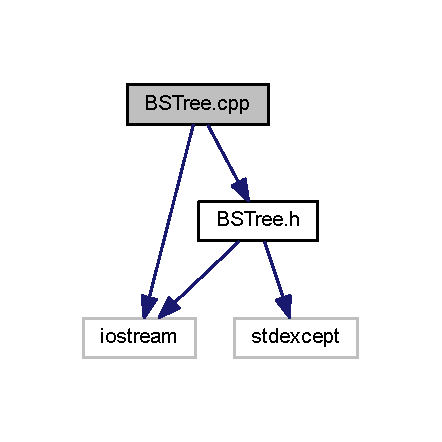
\includegraphics[width=212pt]{_b_s_tree_8cpp__incl}
\end{center}
\end{figure}
This graph shows which files directly or indirectly include this file\+:
\nopagebreak
\begin{figure}[H]
\begin{center}
\leavevmode
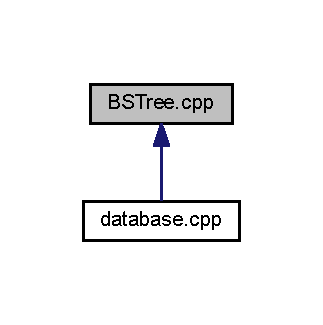
\includegraphics[width=155pt]{_b_s_tree_8cpp__dep__incl}
\end{center}
\end{figure}
\subsection*{Macros}
\begin{DoxyCompactItemize}
\item 
\#define \hyperlink{_b_s_tree_8cpp_a7fc6858eaa479a851625fb1a6913d5df}{B\+S\+T\+R\+E\+E\+\_\+\+C\+PP}
\end{DoxyCompactItemize}


\subsection{Macro Definition Documentation}
\hypertarget{_b_s_tree_8cpp_a7fc6858eaa479a851625fb1a6913d5df}{}\label{_b_s_tree_8cpp_a7fc6858eaa479a851625fb1a6913d5df} 
\index{B\+S\+Tree.\+cpp@{B\+S\+Tree.\+cpp}!B\+S\+T\+R\+E\+E\+\_\+\+C\+PP@{B\+S\+T\+R\+E\+E\+\_\+\+C\+PP}}
\index{B\+S\+T\+R\+E\+E\+\_\+\+C\+PP@{B\+S\+T\+R\+E\+E\+\_\+\+C\+PP}!B\+S\+Tree.\+cpp@{B\+S\+Tree.\+cpp}}
\subsubsection{\texorpdfstring{B\+S\+T\+R\+E\+E\+\_\+\+C\+PP}{BSTREE\_CPP}}
{\footnotesize\ttfamily \#define B\+S\+T\+R\+E\+E\+\_\+\+C\+PP}


\hypertarget{_b_s_tree_8h}{}\section{B\+S\+Tree.\+h File Reference}
\label{_b_s_tree_8h}\index{B\+S\+Tree.\+h@{B\+S\+Tree.\+h}}
{\ttfamily \#include $<$stdexcept$>$}\newline
{\ttfamily \#include $<$iostream$>$}\newline
Include dependency graph for B\+S\+Tree.\+h\+:
\nopagebreak
\begin{figure}[H]
\begin{center}
\leavevmode
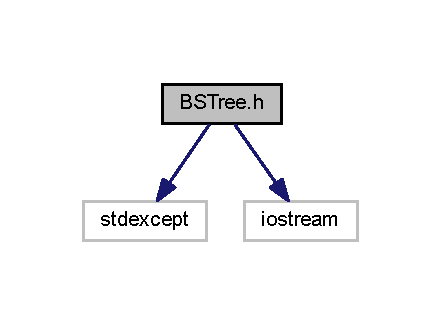
\includegraphics[width=212pt]{_b_s_tree_8h__incl}
\end{center}
\end{figure}
This graph shows which files directly or indirectly include this file\+:
\nopagebreak
\begin{figure}[H]
\begin{center}
\leavevmode
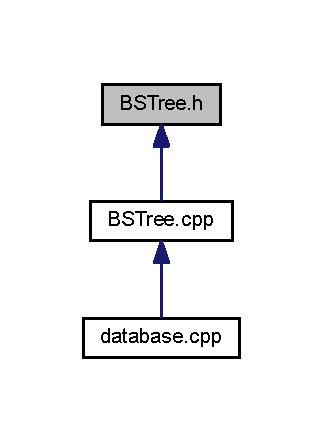
\includegraphics[width=155pt]{_b_s_tree_8h__dep__incl}
\end{center}
\end{figure}
\subsection*{Classes}
\begin{DoxyCompactItemize}
\item 
class \hyperlink{class_b_s_tree}{B\+S\+Tree$<$ Data\+Type, Key\+Type $>$}
\item 
class \hyperlink{class_b_s_tree_1_1_b_s_tree_node}{B\+S\+Tree$<$ Data\+Type, Key\+Type $>$\+::\+B\+S\+Tree\+Node}
\end{DoxyCompactItemize}

\hypertarget{database_8cpp}{}\section{database.\+cpp File Reference}
\label{database_8cpp}\index{database.\+cpp@{database.\+cpp}}
{\ttfamily \#include $<$iostream$>$}\newline
{\ttfamily \#include $<$fstream$>$}\newline
{\ttfamily \#include \char`\"{}B\+S\+Tree.\+cpp\char`\"{}}\newline
Include dependency graph for database.\+cpp\+:
\nopagebreak
\begin{figure}[H]
\begin{center}
\leavevmode
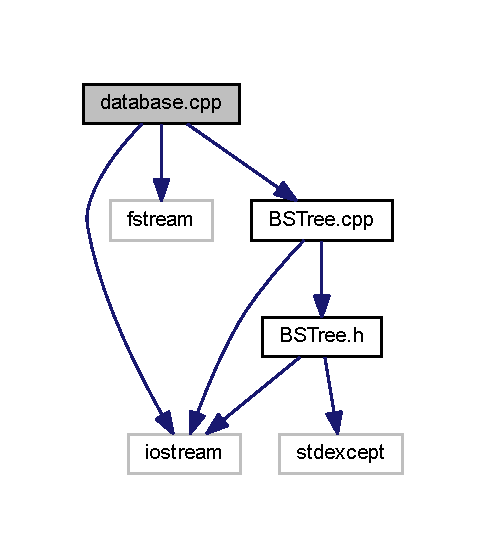
\includegraphics[width=233pt]{database_8cpp__incl}
\end{center}
\end{figure}
\subsection*{Classes}
\begin{DoxyCompactItemize}
\item 
struct \hyperlink{struct_account_record}{Account\+Record}
\item 
struct \hyperlink{struct_index_entry}{Index\+Entry}
\end{DoxyCompactItemize}
\subsection*{Functions}
\begin{DoxyCompactItemize}
\item 
int \hyperlink{database_8cpp_ae66f6b31b5ad750f1fe042a706a4e3d4}{main} ()
\end{DoxyCompactItemize}
\subsection*{Variables}
\begin{DoxyCompactItemize}
\item 
const int \hyperlink{database_8cpp_a5d9687231dabb10b55cd7598e1be6702}{name\+Length} = 11
\item 
const long \hyperlink{database_8cpp_a79deb9c018e75d0dbd8d7e19d0415e89}{bytes\+Per\+Record} = 38
\end{DoxyCompactItemize}


\subsection{Function Documentation}
\hypertarget{database_8cpp_ae66f6b31b5ad750f1fe042a706a4e3d4}{}\label{database_8cpp_ae66f6b31b5ad750f1fe042a706a4e3d4} 
\index{database.\+cpp@{database.\+cpp}!main@{main}}
\index{main@{main}!database.\+cpp@{database.\+cpp}}
\subsubsection{\texorpdfstring{main()}{main()}}
{\footnotesize\ttfamily int main (\begin{DoxyParamCaption}{ }\end{DoxyParamCaption})}


\begin{DoxyCode}
00053 \{    
00054     ifstream acctFile (\textcolor{stringliteral}{"accounts.txt"});   \textcolor{comment}{// "Accounts database file."   }
00055     \hyperlink{struct_account_record}{AccountRecord} acctRec\{\};                \textcolor{comment}{// "Account record."    }
00056     \hyperlink{class_b_s_tree}{BSTree<IndexEntry,int>} index;         \textcolor{comment}{// "Database index."    }
00057     \hyperlink{struct_index_entry}{IndexEntry} entry;                     \textcolor{comment}{// "Index entry."    }
00058     \textcolor{keywordtype}{int} searchID;                         \textcolor{comment}{// "User input account ID."}
00059     \textcolor{keywordtype}{long} record\_num\{\};                          \textcolor{comment}{// "Record number."  }
00060 
00061     \textcolor{comment}{// "Iterates through the database records. This will read the    }
00062     \textcolor{comment}{// account ID and add the (account ID, record number) pair to the    }
00063     \textcolor{comment}{// index."    }
00064     \textcolor{keywordtype}{string} s;
00065     acctFile >> entry.\hyperlink{struct_index_entry_aa5008695f70f365c7959d42ccca0fa13}{acctID};
00066     \textcolor{keywordflow}{while} (acctFile.good())
00067     \{
00068         acctFile >> s >> s >> s;
00069         entry.\hyperlink{struct_index_entry_a3f71077b699f2d718ca60df893c4c470}{recNum} = record\_num;
00070         record\_num++;
00071         index.\hyperlink{class_b_s_tree_a3136c063de9adf6f55e524ad099df62f}{insert}(entry);
00072         acctFile >> entry.\hyperlink{struct_index_entry_aa5008695f70f365c7959d42ccca0fa13}{acctID};
00073     \}
00074     \textcolor{comment}{// "Outputs the account IDs in ascending order."   }
00075     cout << \textcolor{stringliteral}{"\(\backslash\)nAccount IDs in ascending order : "} << endl;
00076     index.\hyperlink{class_b_s_tree_a0f0b3362a2b927092a464cb37edf59b3}{writeKeys}();
00077     \textcolor{comment}{// "Clears the status flags for the database file."    }
00078     acctFile.clear();
00079     acctFile.close();
00080     \textcolor{comment}{// "Reads an account ID from the keyboard and outputs the    }
00081     \textcolor{comment}{// corresponding record."}
00082     acctFile.open(\textcolor{stringliteral}{"accounts.txt"});
00083     cout << endl << \textcolor{stringliteral}{"Enter account ID : "};
00084     \textcolor{keywordflow}{while} (cin >> searchID)
00085     \{
00086         \textcolor{keywordflow}{if} (index.\hyperlink{class_b_s_tree_a464aa205470b150038ff35dfa01d89b8}{retrieve}(searchID, entry))
00087         \{
00088             \textcolor{keywordflow}{for} (\textcolor{keywordtype}{int} i = 0; i <= entry.\hyperlink{struct_index_entry_a3f71077b699f2d718ca60df893c4c470}{recNum}; i++)
00089             \{
00090                 acctFile >> acctRec.acctID;
00091                 acctFile >> acctRec.firstName >> acctRec.lastName;
00092                 acctFile >> acctRec.balance;
00093             \}
00094 
00095             cout << \textcolor{stringliteral}{"Record # : "} << entry.\hyperlink{struct_index_entry_a3f71077b699f2d718ca60df893c4c470}{recNum} << endl;
00096             cout << \textcolor{stringliteral}{"Account ID : "} << acctRec.acctID << endl;
00097             cout << \textcolor{stringliteral}{"First name : "} << acctRec.firstName << endl;
00098             cout << \textcolor{stringliteral}{"Last name : "} << acctRec.lastName << endl;
00099             cout << \textcolor{stringliteral}{"Balance : "} << acctRec.balance << endl;
00100         \}
00101         \textcolor{keywordflow}{else}
00102         \{
00103             cout << \textcolor{stringliteral}{"There is no record with that account ID. Try another one."};
00104 
00105         \}
00106         acctFile.clear();
00107         acctFile.close();
00108         acctFile.open(\textcolor{stringliteral}{"accounts.txt"});
00109         cout << endl << \textcolor{stringliteral}{"Enter account ID : "};
00110     \}
00111 \}
\end{DoxyCode}
Here is the call graph for this function\+:
\nopagebreak
\begin{figure}[H]
\begin{center}
\leavevmode
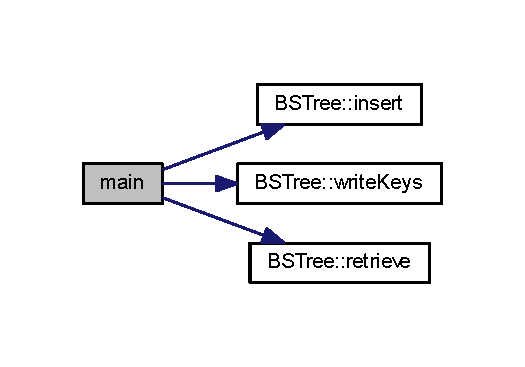
\includegraphics[width=252pt]{database_8cpp_ae66f6b31b5ad750f1fe042a706a4e3d4_cgraph}
\end{center}
\end{figure}


\subsection{Variable Documentation}
\hypertarget{database_8cpp_a79deb9c018e75d0dbd8d7e19d0415e89}{}\label{database_8cpp_a79deb9c018e75d0dbd8d7e19d0415e89} 
\index{database.\+cpp@{database.\+cpp}!bytes\+Per\+Record@{bytes\+Per\+Record}}
\index{bytes\+Per\+Record@{bytes\+Per\+Record}!database.\+cpp@{database.\+cpp}}
\subsubsection{\texorpdfstring{bytes\+Per\+Record}{bytesPerRecord}}
{\footnotesize\ttfamily const long bytes\+Per\+Record = 38}

\hypertarget{database_8cpp_a5d9687231dabb10b55cd7598e1be6702}{}\label{database_8cpp_a5d9687231dabb10b55cd7598e1be6702} 
\index{database.\+cpp@{database.\+cpp}!name\+Length@{name\+Length}}
\index{name\+Length@{name\+Length}!database.\+cpp@{database.\+cpp}}
\subsubsection{\texorpdfstring{name\+Length}{nameLength}}
{\footnotesize\ttfamily const int name\+Length = 11}


\hypertarget{_r_e_a_d_m_e2_8md}{}\section{C\+:/\+Users/15868/\+Documents/\+R\+E\+A\+D\+M\+E2.md File Reference}
\label{_r_e_a_d_m_e2_8md}\index{C\+:/\+Users/15868/\+Documents/\+R\+E\+A\+D\+M\+E2.\+md@{C\+:/\+Users/15868/\+Documents/\+R\+E\+A\+D\+M\+E2.\+md}}

%--- End generated contents ---

% Index
\backmatter
\newpage
\phantomsection
\clearemptydoublepage
\addcontentsline{toc}{chapter}{Index}
\printindex

\end{document}
